\documentclass[titlepage]{article}
\usepackage[utf8]{inputenc}
\usepackage[T1]{fontenc}
\usepackage{graphicx}
\usepackage{hyperref}
\usepackage{breakcites}
\usepackage{float}
\usepackage{textcomp}
\usepackage{amsmath}
\usepackage{textgreek}
\usepackage{authblk}
\usepackage{rotating}
\usepackage{booktabs}
\usepackage{longtable}
\usepackage{pdflscape}
\usepackage{lineno}
\usepackage{xcolor}
\usepackage[
  style=alphabetic,
  citestyle=authoryear,
  backend=biber,
  bibstyle=authortitle,
  doi=true,
  natbib=true,
  sorting=nyt
]{biblatex}
\usepackage{scalerel,xparse}
\usepackage{lineno}

\DeclareFieldFormat{labelalphawidth}{#1}

\bibliographystyle{plain}

\linenumbers

%\addbibresource{TextDataClimateShocks.bib}

% To be able to use emojis
\NewDocumentCommand\emojismile{}{
 \scalerel*{
 
\includegraphics{smiling-face-with-smiling-eyes_1f60a.png}
 }{X}
}

\begin{document}

%https://www.overleaf.com/project/5f918edd1afc380001feca0d
\title{The Effects of Neighborhood Income and Race In Moderating the Effect of Heat on Expressed Mood in the United States}

\author[1,*]{Matthew Cooper}
\author[2]{Jeremiah Osborne-Gowey}
\author[3]{Zheng Liu}
\author[4]{Portia Adade Williams}
\author[5]{Jie Liu}
\author[6]{Aaron Schwartz}
\author[7]{Patrick Baylis} 

\affil[1]{T.H. Chan School of Public Health, Harvard University, Brookline, MA, U.S.A.}
\affil[2]{Environmental Studies Program, University of Colorado Boulder, Boulder, CO, U.S.A.}
\affil[3]{Department of Geographical Sciences, University of Maryland College Park, College Park, MD, U.S.A.}
\affil[4]{CSIR-Science and Technology Policy Research Institute, Accra, Ghana}
\affil[5]{School of Business, East China University of Science and Technology, Shanghai, China} 
\affil[6]{Department of Ecology \& Evolutionary Biology, University of Colorado Boulder, Boulder, CO, U.S.A.}
\affil[7]{Vancouver School of Economics, University of British Columbia, Vancouver, BC, Canada}
\affil[*]{Corresponding Author: mcooper@hsph.harvard.edu, 677 Huntington Ave, Boston, MA 02115}

\date{\parbox{\linewidth}{\centering The authors declare they have no actual or potential competing financial interests.}}

\maketitle

\begin{abstract}

  \textbf{Background} Previous studies have found strong linkages between heat and many indicators of mental health.  However, these studies have not found any heterogeneities in vulnerability based on income or other factors, in spite of the fact that there are strong theoretical reasons to expect the poor and other marginalized groups to be more vulnerable to higher temperates.

  \textbf{Objectives} We tested the hypothesis that the impacts of heat on mental health are heterogeneous based on neighborhood characteristics. 

  \textbf{Methods} We used the expressed mood in 242 million geolocated tweets, paired with census block data on neighborhood characteristics and hourly weather data to test our hypothesis with a segmented regression. 

  \textbf{Results} We found that the effect of heat on expressed mood is much higher in low-income and majority Black neighborhoods.  Additionally, we found that the effects of temperature on mood are greatest in the early morning. 

  \textbf{Discussion} Previous analysis using city-level data have been unable to find heterogeneities in vulnerability to heat, with consequences for our understanding of vulnerability and adaptation.  We present the first evidence of neighborhood heterogeneity in the vulnerability of mental health to heat.  Additionally, examining the timing of impacts of heat on mood suggests that sleep quality plays a role in the effects of heat on mood.

%Higher temperatures associated with climate change are expected to have major impacts on human mental health, and previous work has found strong associations between heat and mental well-being. However, these studies typically use data reported at the city or county level, and, to date, have found no difference in vulnerability based on income or race.  We therefore use expressed mood in a quarter of a billion geolocated tweets as a proxy for mental health status available at fine spatial and temporal scales, and find stark differences in the effects of heat depending on neighborhood characteristics. Here we show that increased temperatures worsen expressed mood in all areas, but that this effect is much stronger in poor and Black neighborhoods. We also find that the effect of heat on expressed mood is greatest in the early morning, supporting the hypothesis that heat affects mental health through a sleep quality pathway. This paper presents the first evidence of neighborhood heterogeneity in the vulnerability of mental health to heat.
\end{abstract}

\section*{Main}
%Overview
Climate change is impacting many aspects of human well-being. A large body of research has explored the ongoing impacts of climate change on agricultural outcomes, economic growth, and physical health \citep{pachauri2014climate}. However, academic and medical researchers have highlighted the relative paucity of empirical studies on the impacts of climate change on mental health \citep{Berry2018Apr, Berrang-Ford2021}. While mental health is under-studied, it accounts for up 13\% of the global burden of disease, representing a major share of total human suffering \citep{Collins2011Jul}, leading to calls for more research into potential linkages between climate change and mental health \citep{Berry2018Apr, Collins2011Jul}. Researchers have begun to answer these calls, finding associations between climate disasters and post-traumatic stress \citep{Schwartz2017Aug}, as well as linkages between higher temperatures and a variety of mental health outcomes \citep{baylis_weather_2018, Mullins2019Dec, Obradovich2018Oct}. Nevertheless, with average global temperatures projected to increase by 1.5\textdegree C within a decade \citep{allen2019technical}, more research is needed into the impacts of increased heat on mental health, especially for identifying the most vulnerable communities.

%Theoretical: frameworks and pathways
Researchers have proposed a number pathways by which temperature can affect mental health \citep{Berry2018Apr, Palinkas2020Apr}. Work on biological mechanisms emphasizes the mental health effects from dehydration and other consequences of maintaining stable body temperature in high heat \citep{Lohmus2018Jul}. Other studies point to linkages between increased temperatures, overall physical health and increases in injuries which can in turn affect mental health \citep{Berry2007}. Additionally, exposure to higher temperatures can affect productivity and income \citep{Burke2015Nov}, leading to second-order impacts on mental health outcomes.

%Empirical: Heat and mental health
Drawing on these frameworks, results from an emerging literature are beginning to document linkages between higher temperatures worsened mental health outcomes. Multiple studies find strong evidence that higher temperatures are associated with increases in suicides in the United States \citep{Burke2018Aug, Mullins2019Dec, Dixon2007May} with other studies finding a similar relationship in locations around the world \citep{Qi2014Dec, Likhvar2011Jan}. Higher temperatures are also correlated with increased hospitalizations related to general mental health issues \citep{Obradovich2018Oct, Mullins2019Dec} and incidents related specific conditions like bipolar disorder and schizophrenia \citep{Lee2007Jan, Sung2013Feb}. Higher temperatures are also linked to increased mortality among people with pre-existing mental health disorders \citep{Hansen2008Oct}.  Finally, recent studies find nighttime temperatures affect sleep quality, with consequences for mental health \citep{Obradovich2017May, Mullins2019Dec}, although these studies have relied on retrospective survey data and have not used data from across the diurnal cycle. 

The effects of heat exposure on mental health are by now relatively well established, yet results from research conducted at national scales indicates surprisingly little heterogeneity in impacts, with consequences for our understanding of groups that are most vulnerable as well as potential adaptations to future heat stress. For example, a large study of temperature and suicide in the USA and Mexico found "no significant difference in suicide response to temperature between rich and poor municipalities or counties" \citep{Burke2018Aug}. Similarly, a national study found no effect of income as modifier of the effect of temperature on suicides, emergency department visits, or self-reported mental health status across the USA \citep{Mullins2019Dec}. A major challenge for these studies, however, is their reliance on data that is typically aggregated to the municipality or county level. As a consequence, these studies are often restricted to between-county metrics of vulnerability and cannot take into account neighborhood effects.

These findings of uniform vulnerability to heat are surprising given that minority groups and low-income people are more likely to be exposed to undesirable temperatures and less able to mitigate the effects of higher heat. For example, people from poorer socio-economic backgrounds are more likely to work outside rather than indoors \citep{Gubernot2014Oct}, more likely to rely on public transportation, bicycling, or walking instead of commuting in their own air-conditioned car \citep{Karner2015Dec}, and more likely to live in housing that is less insulated with poorer quality air-conditioning \citep{Samuelson2020Jun}. Many of these factors that expose low-income people to heat may be exacerbated and compounded for racial minorities. For example, Black Americans face discrimination in employment \citep{Kang2016, Penner2008} and housing access \citep{Desmond2015, Akbar2019}, forcing them into jobs and homes that may expose them to more heat. Additionally, policymakers have historically been less likely to take measures to address environmental hazards in Black neighborhoods \citep{Banzhaf2019}. Some studies find large differences in vulnerability between neighborhoods for a variety of impacts of heat on physical and mental health \citep{Belanger2015Mar, Uejio2011Mar}, as well as for vulnerability to other types of climate shocks like hurricanes \citep{ferre2019hurricane, Gruebner2015Jun}. Thus, there are theoretical reasons to expect heterogeneity in the impact of heat on mental health outcomes for different populations, particularly where socioeconomic, racial and other social inequities intersect, although there is little evidence of this to date. 

While public health data on mental health outcomes is not available at the neighborhood scale, spontaneous, in situ data from the social media platform Twitter can provide an important, inexpensive and timely proxy for mental health at extremely precise spatial and temporal scales. Many studies use the mood expressed in social media posts as an indicator of mental health and well-being \citep{Edo-Osagie2020Jul, Sinnenberg2016Dec}. For example, studies have used Twitter data to identify the onset of Post Traumatic Stress Disorder (PTSD) in individuals even before their formal diagnosis \citep{Reece2017Oct}. Similar methods applied to posts on Facebook can predict the onset of depression \citep{Eichstaedt2018Oct}. In London, day-to-day changes in mental health indicators derived from the text of tweets were associated with changes in mental health crisis episodes \citep{Kolliakou2020Feb}. Across the USA, more positive tweets are associated with a variety of metrics of human well-being \citep{Mitchell2013May}, and twitter has provided insight into population-level patterns of happiness over the course of the day \citep{Dodds2011}. Finally, the mood expressed in tweets has been strongly associated with local weather conditions and air quality \citep{baylis_weather_2018, Zheng2019} and been used as evidence to support the temperature-suicide relationship \citep{Burke2018Aug}. Thus, posts on Twitter provide an proxy for mental health at fine enough spatial scales to examine neighborhood effects on vulnerability to higher temperatures. To explore how neighborhood conditions affect the relationship between heat and mental heath, we draw on a data set of 243 million geolocated tweets from across the continental United States covering the period 2009-2019, each paired with data on local weather and neighborhood conditions.

\section*{Methods}
% from NCC: methods section should be written as concisely as possible and "typically do not exceed 3,000 words"
\subsection*{Tweets \& Mood}
We used data from 243 million geo-located English-language tweets from the continental United States from the years 2009 to 2019. The data were collected by the University of Vermont through a special agreement with Twitter, and represent a random sample from the population of geolocated tweets.  The Twitter data consists of publicly posted messages, or tweets, that are short status messages users post to the platform. We only considered users’ original content, thus did not include retweets in our analysis. Additionally, we excluded all tweets that contained weather-related terms, to ensure that the mood expressed in the tweets was reflective of a user's mental state, and not a commentary on the weather.

Expressed mood is a widely used metric to assess mental health and well-being from posts on social media platforms. We use the VADER metric to assess the mood of Twitter posts as it was specifically designed for microblogs like Twitter \citep{hutto2014vader}. The VADER (Valence Aware Dictionary for Sentiment Reasoning) corpus \citep{gilbert_vader_2014} is a lexical, rule-based sentiment analysis tool that is specifically attuned to moods expressed on social media and includes several features, as:

\begin{itemize}
 \item Incorporating lexical features common to informal media, such as slang (``sux"), and acronyms (``lol").
 \item Negations (``\textit{not} good", ``\textit{wasn't} bad")
 \item Punctuation (``Good!!!")
 \item Word shape, such as capitalization (``The movie was AMAZING")
 \item Emoticons and emojis (``:-)", ``\emojismile")
 \item Degree modifiers (``very excellent" or ``kind of crappy")
\end{itemize} 

The VADER method yields a value for the mood of a tweet, with a score of 0 for neutral tweets, a score $> 0$ for positive-mood tweets and a score $< 0$ for negative-mood tweets. While we ultimately settled on using VADER for assigning sentiment scores, we also conducted analyses using the Hedonometer and AFINN mood analysis methods, with similar results (See Supplement).

\subsection*{Weather}
We used data on local weather conditions from the North American Land Data Assimilation System (NLDAS), a gridded product developed by several collaborative institutions, including NOAA, NASA, Princeton University, and the University of Washington. This dataset is available at an hourly temporal resolution, and at 1/8th decimal degree spatial resolution, and integrates a large quantity of observation-based and modeled data \citep{xia_continental-scale_2012}. We extracted temperature, specific humidity, air pressure, total precipitation, shortwave radiation, and wind speed for the exact hour and location of each tweet. 

We calculated the Wet Bulb Globe Temperature (WBGT) at the time and location of each tweet. The WBGT is the temperature that a wet globe thermometer would read in direct sunlight, and gives a reading lower than a dry bulb temperature due to evaporative cooling. The WBGT can be estimated given normal temperature, relative humidity, solar radiation, and wind speed. Because evaporative cooling is how humans cool themselves through perspiration, this temperature better indicates the heat stress that people are experiencing \citep{budd2008wet}. Metrics like WBGT that account for the effects of humidity and other factors on heat stress have been associated with diminished economic output \citep{rao2020projections}, increased crime \citep{hu2017impact}, increased mortality \citep{chien2016spatiotemporal, armstrong2019role}, and worsened mental health outcomes \citep{vida2012relationship, ding2016importance}.

We derived relative humidity using methods described by Bolton et al. \citep{bolton_computation_1980} which use temperature, specific humidity, and pressure. We then calculated the WBGT using the formula described by Heo et al. \citep{heo2019comparison}.  Throughout the paper we give the median dry bulb temperature observed at each given wet bulb temp degree across our data set. It should be noted, however, that a wide range of dry bulb temperatures can be associated with a given wet bulb globe temperature, depending on humidity, wind speed, and sunlight.

\subsection*{Socio-Economic Data}
We used data from the American Community Survey (ACS) administered by the US Census to estimate income levels and the racial composition of neighborhoods where tweets were located. Data was at the level of the census block group, the smallest unit for which the US Census releases public data. Following Census categories, we report racial characteristics of neighborhoods as majority population of four broad racial categories - non-Hispanic Black, non-Hispanic white, Hispanic of any race, and other, which includes Native American, multi-racial, Asian-American and Pacific Islander. 

The ACS data covers five-year periods. We therefore matched each tweet with census block group data from the year at the middle year of each survey's five-year range. For example, tweets from 2014 were matched to data from the 2012-2016 ACS. Because the most recent available ACS was from 2014-2018, all tweets from year years greater than 2016 were matched to this dataset. We used data from the Integrated Public Use Microdata Series (IPUMS USA) National Historical Geographic Information System (NHGIS) service provided by the University of Minnesota \citep{ruggles2018ipums}.

We use the mean annual income per capita from the ACS, standardized so that values for each year are in 2019 dollars. For racial categories, we combined the various categories provided by the ACS into four racial groups: non-Hispanic white, non-Hispanic Black, Hispanic of any race, and an "other" category for non-Hispanic people who were neither Black nor white, such as Asian, Native American, or mixed-race people.

We present income and percentiles based on the observed percentiles across all tweets in our data set.
 
\subsection*{Modeling}
We assessed how expressed mood is affected by Wet Bulb Globe Temperature using segmented regressions, controlling for precipitation, shortwave solar radiation (sunshine), as well as the following spatio-temporal fixed effects: day of the week, time of day, day of the year, year, month, and county. 

Our initial model (for Fig. \ref{fig:wbgt}) takes the following form:

\begin{equation}
 y = \beta_0 + f_t(t) + \beta_p p + \beta_s s + \Phi + \epsilon
 \label{mod:1}
\end{equation}

Where $y$ is the mood of a tweet, $t$ is the wet bulb globe temperature at the hour of the tweet, $p$ is a binary variable indicating whether it rained at the hour of the tweet, $s$ is the incoming shortwave radiation, or sunshine, in $W/m^2$, at the hour of the tweet, $\Phi$ is the spatio-temporal fixed effects, $\epsilon$ is the normally-distributed errors, and $f_t$ represents the segmented effect for $t$, with knots at -10\textdegree, 0\textdegree, 5\textdegree, 10\textdegree, 15\textdegree, 20\textdegree, and 25\textdegree C WBGT. We estimate the 95\% confidence interval of all our models using 80-fold bootstrapping. 

To examine how income and racial groups moderate the effect of heat on mood, we extend our model to the following form:

\begin{equation}
 y = \beta_0 + f_t(t) + f_{mt}(m t) + \beta_p p + \beta_{mp} m p + \beta_s s + \beta_{ms} m s + \Phi + \epsilon
 \label{mod:2}
\end{equation}

Where $m$ is either the log-transformed average income in the census block where the tweet originated, or a dummy variable for the four racial categories. We specify alternative models where income is a dummy variable in three bins and were race is a continuous variable for the percent of a census block population that is white These alternative specifications yield similar results. We also examine the effects of rainfall and sunshine on mood by income and race. These alternative specifications and analysis of rainfall and sunshine effects are available in the Supplement.

Finally, we fit a model for how heat affects mood by time of day. For this analysis, we used a varying-coefficient model, where the effect of heat is linear, but the coefficient for the effect varies non-linearly as a function of the time of day. Because we modeled the effect of heat as linear, we excluded all tweets with an observed temperatures less than 5\textdegree C WBGT so that we were only including values at which our previous analyses suggested the heat-mood relationship is monotonic. This final model took the following form:

\begin{equation}
 y = \beta_0 + f_h(h)t + \beta_p p + \beta_s s + \Phi + \epsilon
 \label{mod:tod}
\end{equation}

In this final model, $f_{h}$ is the coefficient for temperature, $t$, and varies non-linearly by time of day, $h$. To ensure that the effect $f_{h}$ is cyclical, we estimated $f_{h}$ using 2nd-order B-splines, also known as a tent function basis \cite[Chapter~4.2]{wood2017generalized}, with knots every two hours.

\section*{Results}

\subsection*{Effect of Heat on Sentiment}
We examine the relationship between the mood expressed in tweets and the prevailing Wet Bulb Globe Temperature (WBGT), a temperature metric that accounts for dry-bulb temperature, humidity, wind speed, and solar radiation to more accurately describe the effects of heat on the human body \citep{budd2008wet}. We find higher temperatures are associated with worsened mood (Fig. \ref{fig:wbgt}) after controlling for a variety of fixed effects across all tweets. Mood is highest at 5\textdegree C WBGT (associated in our data set with a median dry bulb temperature on 12\textdegree C/54\textdegree F) with the largest declines between 20\textdegree -25\textdegree C WBGT (dry bulb 29\textdegree-36\textdegree C/84\textdegree-97\textdegree F). Mood also declines with colder temperatures (below 5\textdegree C WBGT), although only slightly. Dis-aggregating our analysis by metropolitan area and using alternative methods to estimate expressed mood all yield similar results (see Supplement).

\begin{figure}[H]
 \centering
 \includegraphics[width=\linewidth]{Xfigure1.pdf}
 \caption{Relationship between Wet Bulb Globe Temperature (WBGT) and expressed mood in tweets. As temperatures increase above 5\textdegree C WBGT, mood rapidly declines.  Shaded area shows the 95\% confidence interval estimated with bootstrapping.}
 \label{fig:wbgt}
\end{figure}

We find that mean neighborhood income strongly moderates the relationship between temperature and mood (Fig. \ref{fig:hetero}), with large differences in mood between the poorest (5th percentile) and wealthiest (95th percentile) neighborhoods. As temperatures increase to a modest 20\textdegree C WBGT (29\textdegree C/84\textdegree F), mood increases in the wealthiest neighborhoods but decreases in the median and lowest income neighborhoods. The wealthiest neighborhoods do not see decreases in mood until temperatures exceed 20\textdegree C WBGT (29\textdegree C/84\textdegree F), at which point mood decreases relatively evenly regardless of neighborhood income percentile.

We also explored how neighborhood racial characteristics affect the relationship between temperature and mood, and we find the effects of heat are felt disproportionately in neighborhoods that are majority Black (Fig. \ref{fig:hetero}). Relative to an optimum temperature of 5\textdegree C WBGT (12\textdegree C/54\textdegree F), as temperatures increase to 30\textdegree C WBGT (42\textdegree C/108\textdegree F), the mood of tweets in majority Black neighborhoods decrease four times as much as the mood of people in other neighborhoods. Additionally, at mild to warm temperatures of 10\textdegree C WBGT (19\textdegree C/66\textdegree F) to 25\textdegree C WBGT (36\textdegree C/97\textdegree F), people in majority Hispanic neighborhoods have slightly lower mood than people in majority white or other neighborhoods, although this gap narrows at higher temperatures.

\begin{figure}[H]
  %\makebox[\textwidth][c]{\includegraphics[width=1.4\textwidth]{Xfigure2.pdf}}
  \includegraphics[width=\textwidth]{Xfigure2.pdf}
  \caption{Effect of changes in WBGT on expressed mood as moderated by neighborhood income (a) and race (b). Shaded area shows the 95\% confidence interval estimated with bootstrapping.}
\label{fig:hetero}
\end{figure}

\subsection*{Comparison With Other Events}
We compared the expressed mood from exposure to temperatures to two other events associated with impacts on mood and other mental health outcomes: the weekly change from Saturday to Monday, as well as the impact of a major natural disaster (see Fig. \ref{fig:compare}). For this comparison, we define heat impact as the changes in mood associated with temperatures increasing from 5\textdegree C WBGT (12\textdegree C/54\textdegree F) to 25\textdegree C WBGT (36\textdegree C/97\textdegree F); we define weekly changes as the difference between the mean Saturday mood and the mean Monday mood, calculated across the entire data set; and we define the impact of Hurricane Sandy as the change in mood from the week before the hurricane made landfall to the week after, calculated for only impacted counties. Both of these events are associated with mental health impacts: the decrease in expressed mood on Twitter from Saturdays to Mondays mirrors mirrors the weekly dynamics of suicide rates \citep{CDC2021}, while Hurricane Sandy was associated with mental health effects on victims including increased anxiety, PTSD, and depression \citep{Schwartz2017Aug, Lieberman-Cribbin2017}.

\begin{figure}[H]
 \centering
 \includegraphics[width=\linewidth]{Xfigure3.pdf}
 \caption{Decline in mood as temperature changes from mild (5\textdegree C WBGT) high (25\textdegree C WBGT) across different neighborhood types, compared with the impacts of the change from Saturday to Monday, as well as the change associated with Hurricane Sandy.  Error bars show the 95\% confidence interval estimated with bootstrapping.}
 \label{fig:compare}
\end{figure}

We find that the decline in mood in wealthier and majority white neighborhoods from exposure to increasing temperatures is less than the average weekly change in mood from Saturday to Monday (see Fig. \ref{fig:compare}). Conversely, the effects of exposure to increasing temperatures in poorer and majority Black neighborhoods are much larger than the average weekly change in mood. Additionally, the impacts of exposure to these changes in temperature for the more vulnerable neighborhoods are close in severity to the impact on mood from experiencing a major hurricane.

\subsection*{Effect of Heat by Time of Day}
In addition to providing data with high spatial resolution, Twitter data also comes with very high temporal resolution as each tweet is time-stamped. Thus, we were able to examine the impact of heat on mood over the course of the day (Fig. \ref{fig:ts-wbgt}). We found that heat is associated with improved mood for a brief period in the late morning, and then has a negative effect on mood during the latter half of the day, with a consistent effect from noon until 9pm. This effect weakens in the early evening through midnight, and then increases substantially throughout the night. Heat has the greatest effect on expressed mood at 6am, an effect over twice as large as during the day.

\begin{figure}[H]
 \centering
 \includegraphics[width=\linewidth]{Xfigure4.pdf}
 \caption{Effects of rising temperatures on mood by hour of the day, with a 95\% confidence interval. The value shown is the predicted change in VADER score for a 10\textdegree C WBGT increase in temperatures. Shaded area shows the 95\% confidence interval estimated with bootstrapping.}
 \label{fig:ts-wbgt}
\end{figure}

\section*{Discussion}
% Compare weekly changes in mood to weekly changes in suicides
We found that the change from an optimum temperature to a higher temperature is associated with an overall decrease in mood similar in magnitude to the degree of change in mood from Monday to Saturday, a weekly change associated with an increase in suicides of 23\% over the course of the study period \citep{CDC2021}, and that the same level of heat in a poor or Black neighborhood is associated with a change in mood nearly matching the impact of a major Hurricane, an event associated with suicides and PTSD \citep{Schwartz2017Aug, Lieberman-Cribbin2017}.  Thus, while research on linkages between expressed mood and other mental health outcomes like suicides and hospitalizations is still nascent, there are clear similarities in patters of expressed mood and mental health at specific time scales and following certain events.  This suggests that the changes in expressed mood we observe at neighborhood scales is indicative of other mental health outcomes such as suicides and hospitalizations.

% Discuss the NOVELTY: quote Burke and Mullins, refute their interpretations, people have said XX, but we have shown ~XX.
% Variations in vulnerability also indicates ADAPTATION
Previous work conducted with county-scale data found no heterogeneity in mental health vulnerability by income. Such analyses have led to conclusions that the mental health effects of climate change will be uniform, least in developed countries, and that adaptation with technologies like air-conditioning will not mitigate the mental health effects of climate change. For example, Mullins et al. conclude that ``individuals have not been able to successfully reduce the negative effects of higher temperatures on mental health" \citep{Mullins2019Dec}. Contrary to these analyses, we found large heterogeneity in vulnerability by neighborhood racial composition and per-capita income. This suggests that the mental health effects of climate change will not be uniform and, like other impacts, will fall disproportionately on the vulnerable and marginalized. More positively, it does suggest that adaptation is possible, and, for communities with infrastructure and working conditions similar to those of higher-income Americans, the effects of high temperatures on mental health may be addressable.

Examining the role of race in vulnerability, we find that majority Black non-Hispanic neighborhoods are much more affected by higher temperatures than neighborhoods with a non-Black majority. Surprisingly, we did not find an effect for people with Hispanic ethnicity, given that Hispanic peoples can be marginalized in employment and housing. These findings may be because the ethnic category of Hispanic is more broad and encompasses many more groups with more diverse histories and living conditions than Black Americans. It may also be due to that fact that more marginalized and heat-vulnerable Hispanic people were more likely to tweet in the Spanish language, which we did not include our analysis. Additionally, there are many other marginalized groups in the United States, particularly indigenous people, that we did not have sufficient data to examine with respect to heat and mental health. Examining the effects of both race and income, we find that race is more important for vulnerability than income. This probably due in part to the fact that Black Americans have historically been forced through redlining into neighborhoods with fewer trees that are much more impacted by heat \citep{Hoffman2020, Locke2021}.  This suggests that racism and patterns of housing discrimination contribute to making Black Americans more vulnerable to heat, even at similar levels of income as other groups, and that reducing existing discrimination in housing and employment is an important adaptation strategy.

% Connect to bigger literature on vulnerability
This study shows the importance of examining heterogeneities in vulnerability in analyses of climate change impacts.  Additionally, it shows how measuring outcomes at fine spatial scales necessary for understanding how factors like race and income matter for vulnerability \citep{Tong2021}. Even within a relatively wealthy nation, we find that high temperatures affect certain populations to the same degree as a major hurricane. Thus, it is likely that heat waves have a much greater mental health impact throughout the developing world, where temperatures are expected to be much higher \citep{Raymond2020May}, heatwaves are already under-counted \citep{Harrington2020Sep}, and adaptive technologies like air conditioning are more scarce \citep{Biardeau2020Jan}.

In addition to exploring heterogeneities in vulnerability, using twitter data lets us explore how the effect of heat varies by time of date and infer possible important pathways in the heat-mental health relationship. Recent research has suggested that the impacts of heat on sleep quality may play a large role in the observed mental health effects of heat \citep{Obradovich2017May, Mullins2019Dec}, and our temporal analysis largely supports this hypothesis.  We found much stronger effects of heat on expressed sentiment in the early morning, adding weight to the sleep quality pathway linking heat and mental health that other authors have found.  This suggests that efforts to improve mental health during heat waves may have the largest impact by focusing on providing electricity and air conditioning at night.


% Caveats
% Mood is a fuzzy indicator but we have BIG DATA
While these findings are robust to different model specifications and metrics of mood, there are important considerations in this analysis.  One caveat associated with this data is that we were only able to locate the tweets within the census block from which the tweet was sent, and in some cases the income level of a census block may be only weakly indicative of the wealth of the people who are found that census block. For example, some public spaces are estimated to have very low income levels even though people from a variety of income levels may occupy those spaces throughout the day. These issue may in fact lead us to under-estimate the true effect of heat on mental health for poor and Black people. Another issue with using Twitter data is that, while Twitter is used by more than one in five Americans and at similar rates across racial groups, Twitter users may not be representative of the general population, as they are typically younger, wealthier, and more educated \citep{Pew2020Sep}. Nevertheless, we found a large volume of tweets across all neighborhood types.

% NCC doesnt have a "conclusion" section, but this is intended as an overall summary paragraph
While climate change will have widespread and severe impacts on human well-being, our work emphasizes just how unevenly these impacts will be distributed. People with more money, access to aid and infrastructure, and who belong to ethnic groups in power are less affected by climate shocks and natural disasters and more able to adapt \citep{bullard2012wrong}. While the physical health impacts of these shocks are more visible and easy to measure, the mental health impacts of climate change are also causing severe human suffering and there is no reason to believe they will not also be highly unevenly distributed. Thus, there are strong theoretical priors behind the hypothesis that low-income and marginalized people are more vulnerable to the mental health impacts of higher temperatures, even though previous work at coarse spatial scales had not found such an effect. By using fine-scale Twitter data, we show that there are indeed stark differences in the mental health impacts of heat among neighborhoods in the United States. These findings have significant implications for urban planning, climate and environmental justice, and mental health.

\section*{Acknowledgements}
%Official SESYNC wording
This work was supported by the National Socio-Environmental Synthesis Center (SESYNC) under funding received from the National Science Foundation DBI-1639145. Additionally, computational resources for this project were provided for the Microsoft Azure cloud through Microsoft's AI for Earth program.

This data came from Twitter via the University of Vermont’s (UVM) agreement with Twitter to access its streaming API - colloquially referred to as the Decahose. The UVM special agreement with Twitter allows for access to this data for research and analysis purposes and this work complies with all the terms of service for Twitter and UVM. 


\section*{Author Contributions}
Author contributions: M.C., J.O.-G., A.S. and P.B. designed the research and modeling strategy; A.S. provided data; M.C and Z.L. prepared data; M.C. and J.O.-G. analyzed data; and M.C., J.O.-G., P.A.W., and J.L. wrote the paper.

\noindent This paper was the result of a SESYNC graduate pursuits project co-lead by M.C. and J.O.-G.

%\printbibliography
\documentclass{article}
\usepackage{graphicx}
\usepackage{hyperref}
\usepackage[a4paper, margin=1.25in]{geometry}
\usepackage{breakcites}
\usepackage{subcaption}
\usepackage{float}
\usepackage{textcomp}
\usepackage{amsmath}
\usepackage{textgreek}
\usepackage{authblk}
\usepackage{rotating}
\usepackage{booktabs}
\usepackage{longtable}
\usepackage{pdflscape}
\usepackage{lineno}
\usepackage{xcolor}
\usepackage[
  style=numeric,
  citestyle=numeric-comp,
  backend=biber,
  doi=true,
  natbib=true,
  sorting=none
]{biblatex}

\addbibresource{TextDataClimateShocks.bib}

\begin{document}
%https://www.overleaf.com/project/5f918edd1afc380001feca0d
\title{Fine-scale Twitter Big Data Reveals Neighborhood Inequalities in Mental Health Effects of High Temperatures}

\author[1, *]{Matthew Cooper}
\author[2]{Jeremiah Osborne-Gowey}
\author[3]{Zheng Liu}
\author[4]{Jie Liu}
\author[5]{Portia Adade Williams}
\author[6]{Aaron Schwartz}
\author[7]{Patrick Baylis}

\affil[1]{T.H. Chan School of Public Health, Harvard University}
\affil[2]{University of Colorado Boulder}
\affil[3]{Department of Geographical Sciences, University of Maryland College Park}
\affil[4]{School of Business, East China University of Science and Technology}
\affil[5]{University of Cape Town}
\affil[6]{University of Colorado Boulder}
\affil[7]{University of British Columbia}
\affil[*]{Corresponding Author: mcooper@hsph.harvard.edu}

\maketitle

\begin{abstract}
%Limit 150 words: https://www.nature.com/nclimate/about/content
%Actually there are lots of examples of articles with > 150 words, but I think we should keep it concise
Higher temperatures associated with climate change are expected to have major impacts on human mental health.  Indeed, traditional analyses of heat and mental health outcomes using data collected by public agencies have found associations between elevated temperatures and increases in outcomes such as suicides and mental-health related hospitalizations.  However, these studies, which typically use data reported at the city or county level, have found no difference in vulnerability based on income.  We overturn this finding and show that there are stark differences in vulnerability using a novel data source: expressed sentiment in 250 million geolocated tweets, matched with prevailing weather as well as neighborhood economic and demographic conditions.  We find that increased temperatures worsen expressed sentiment in all areas, but that this effects is much stronger in poor and black neighborhoods.

\end{abstract}

Keywords: Text Data, Environmental Shocks, Social Media Mining, Sentiment Analysis, Topic Modeling, Social Media, Public Opinion, Perception, Sentiment, Media, News, Twitter, Climate Change, Science Communication, Policy, Planning, Methods, Text Mining, Natural Language Processing, NLP, Latent Dirichlet Allocation, LDA, Political Ecology, Politics, Resilience, Adaptation, Suicide, Mortality, Morbidity, Self-harm, 

    
%Cite this new paper: https://doi.org/10.1016/S2542-5196(20)30251-5
% And: https://eos.org/articles/long-term-drought-harms-mental-health-in-rural-communities and this is the conf. paper citation https://agu.confex.com/agu/fm20/meetingapp.cgi/Paper/771750
\section{Introduction}

% Organize as follows:

% Heatwaves are known to worsen mental health
% AND mental health is strongly associated with income
% AND wealthier better able to cope with heatwaves 
% BUT we know little about the interaction between heatwaves, mental health and income
% THEREFORE: we did this really novel study.

% Jeremiah Osborne-Gowey: Randy Olsen (of "Don't be such a scientist" fame) and his ABT - And But Therefor framework for communicating - https://www.huffpost.com/entry/and-but-therefore-randy-o_b_8813330
% Jeremiah Osborne-Gowey: https://blogs.scientificamerican.com/observations/how-the-word-but-could-save-the-world/


This work builds on existing work by \citep{baylis_weather_2018}. 




%Intro Paragraph
% I think this should be more about climate change and mental health broadly, as well as a bit about how income has been theorized to affect vulnerability, but there is no evidence yet.  This can be shorter as well, as we have a lot of detail in the Background section 
% Cite this high-level study: https://www.nature.com/articles/s41558-018-0102-4/
% Also this review article saying more research is needed https://www.sciencedirect.com/science/article/pii/S0033350618302130
% -Matt

Research has shown strong linkages between ambient environmental conditions and mental health, with extreme temperatures  frequently associated with poorer overall mental health. Individual's mental health is strongly associated with income with people in lower income levels frequently experiencing higher stress levels and less able to find help for coping with these stresses. Other research on how people cope with environmental temperature extremes indicate that wealthier are better able to cope with heatwaves, whether from traveling to cooler climes, accessing air conditioning, or other temperature ameliorating strategies that may require access to financial capital. Yet we know relatively little about the interaction between temperature, mental health and income. Furthermore, previous studies that did attempt to examine relationships between environmental extremes and health sometimes aggregated data at scales too coarse to examine whether income may be an ameliorating factor. This study examines the interactions between these three using relatively fine-scale, publicly available data. Our research expands on existing studies of temperature and sentiment - one measure of mental health - by examining finer-scale data and incorporating income data to examine correlations between temperature extremes and sentiment.

Human moods and mental states are important aspects of overall well-being and can be influenced by ambient, persistent and fluctuating environmental conditions. Climate change is accelerating the rate and variability around meteorological norms like the timing, magnitude, intensity and duration of precipitation events and air temperature minima and maxima \href{https://www.ipcc.ch/site/assets/uploads/2018/03/SREX-Chap3_FINAL-1.pdf}{(link)}. Previous work \citep{baylis_weather_2018} indicate important linkages between human mood and meterological conditions. Previous analyses of the effects of weather on mood (as expressed in sentiment of text-based message), however, were constructed at the aggregated city/day level and did not account for differences in socio-economic status which may affect access to resources (e.g., air conditioning) that can offset the effects of exposure to temperature extremes. Here, we build on these previous studies by examining the hourly effects of weather on human sentiment, an expression of mood, exploring geographic and economic heterogeneity at a finer-scale resolution than previous studies.  


\section{Background}
\subsection{Temperature and Mental Health}
%Jeremiah Osborne-Gowey: We report on physiological and mental health in text here. Maybe just a heading of "health"?
%I think physical health is beyond the scope of this paper -Matt

%https://www.pnas.org/content/115/43/10953
Higher temperatures are associated with many indicators of worsened mental health.  Multiple studies have found strong evidence that higher temperatures are associated with increases in suicides in the United States \citep{Burke2018Aug, Mullins2019Dec, Dixon2007May}, and many others have demonstrated the same relationship around the world \citep{Qi2014Dec, Page2006Aug, Likhvar2011Jan}.  In addition to suicide, other research has found effects temperature on hospitalization events related to mental health disorders such as bipolar disorder and schizophrenia \citep{Mullins2019Dec, Lee2007Jan, Shapira2004Feb, Sung2013Feb, Gupta1992Jun, Hansen2008Oct}.

Temperature has been hypothesized to impact mental health through a number of pathways.  Work on biological mechanisms emphasize that there may be mental health effects from maintaining stable body temperature in high heat \cite{Lohmus2018Jul}.  Additionally, recent studies have found that nighttime temperatures affects sleep quality \citep{Obradovich2017May, Mullins2019Dec}

% The pathways
Higher temperature associated with climate change could influence mental health directly by exposing people to trauma. It could also indirectly influence mental health by affecting (1) physical health and (2)community wellbeing\citep{RN1314}. For the direct influence pathway, extreme heat events or increasing temperatures have been associated with the increase in aggression,higher suicide rates and other hospital admissions(Anderson and Anderson 1998,Cheatwood 1995; Cohn et al. 2004,Bouchama et al.2007.). Heat exposures in working environments could also reduce people's capacity to deal with physical and mental task, and increase the risk of accidents, because of the excessive core body temperature and dehydration((Bridger 2003; Kerslake 1972; Kjellstrom et al.2009d,Leithead and Lind 1964,Schrier et al. 1970). The loss of work capacity would in turn result in loss of income, which could also cause mental health problems(Kjellstrom 2009b).%% more physiological terms 

As for the indirect pathway, first, because of the reciprocal causation relationship between physical health problems and mental health problems(Miller et al. 2009; Prince et al. 2007), heat exposures associated with climate change along with other climate events and indirect health risks threatening physical health will directly influence mental health((Berry 2007,World Health Organization 2008b). Second,disordered temperature associated with climate change may destroy the economic in agricultural-production-dependent communities. For example, extreme heat reduces the work capacity of laborers in farm fields(Kjellstrom et al. 2009d), which further destroys agricultural-supported industries in local area(Berry et al. 2008). The following economic pressures would undermine social capital and then lead to mental health problems.

% Heatwaves are known to worsen mental health



https://doi.org/10.1016/j.puhe.2018.06.008 (review study - will have more to cite)
https://www.nature.com/articles/s41558-018-0222-x
https://ehp.niehs.nih.gov/doi/full/10.1289/ehp.11339
https://ijmhs.biomedcentral.com/articles/10.1186/s13033-018-0210-6
https://www.nature.com/articles/s41558-018-0102-4/
https://doi.org/10.1016/j.jhealeco.2019.102240

[ADD SUICIDE DATA TO HEALTH SECTION?]
https://www.psychologytoday.com/us/blog/greening-the-media/201809/global-warming-and-suicide

\subsection{Mental Health and Vulnerability}
% This is good, but probably should be shortened.  Maybe one para showing that income matters, one para discussing pathways, also maybe focus/change phrasing to be more on "vulnerability" -Matt

% AND mental health is strongly associated with income
% 1)Childhood 2)adulthood 3)gender
% Perceived income level

% Talk more about race
% This is interesting: https://www.pnas.org/content/118/17/e2019624118.abstract?etoc

The relationship between income, socioeconomic status (SES), well-being and mental health is one of the strongest established patterns in psycho-social literature \citep{Easterlin1974Jan, holzer1986increased, Perry1996Sep} (I cant find Ng et al. 2014). Much of the research into these patterns focuses on the inequalities and distribution of the effects on individual well-being. Subsequent work on mental health outcomes, one measure of well-being, have established strong associations between SES, income and mental health with the most and least privileged most commonly associated with the best and worse mental health experiences and outcomes, respectively \citep{Sevenson2008Aug}(cites: Ng et al. 2014). 

For example, results from a cross-sectional comparative study of socioeconomic factors and use of mental health services by people living in Ontario, Canada and the United States, indicate clear disparities in use of mental health services between those with the highest income levels and lowest mental health morbidity and those with the lowest income levels and highest mental health morbidity - those with higher incomes tended to have lower mental health morbidity issues while utilizing mental health services more than those with lower incomes and higher mental health issues \citep{Katz1997}. 

Results from a systematic review of the literature on associations between social inequalities and mental health disorders indicate a clear and prevailing link between  one or more indicators of less social privilege and higher prevalence of mental health disorders \citep{Fryers2003}, with low income one of the most consistent markers of and associations with increases in common mental health disorders. Collectively, results from the income and mental health literature indicate that socially disadvantaged populations experience significantly more frequent common mental health disorders. Scholars use mental health disparities to indicate the disproportionate amount of mental health disorders among persons of low SES \citep{RN1292}

The established association between poverty and mental health revealed that that income distribution may have a significant influence upon mental health over and above the effect of poverty \citep{HANANDITA201459}.Poverty has been identified as one of the major risk factors in mental health. For instance, some systematic reviews have shown that socioeconomically disadvantaged children and adolescents were 2-3 times more likely to have mental health problems than others\citep{REISS201324}, while the household increases in financial resources are generally associated with an overall reduction of mental health problems\citep{2015Does}. Others have argued that increases in SES can serve as a buffer against the negative impacts of difficult life experiences on mental health, particularly for individuals already under substantive mental stress \citep{Kawachi2001Sep}. Thus, SES and income are associated with mental health improvements in SES and income can serve to decrease mental health problems.

 
Several reasons could explain why poverty may effect mental health. 1) the “social causation hypothesis” which suggests that stress or deprivation or decreasing the likelihood of people getting treatment may lead to poor mental health\citep{mills2015}, while social capital could reduce the likelihood of living in poverty and reduces the risk of mental disorders such as depressive symptoms and suicidal tendencies\citep{RN1291}. 2) negative life events in a person’s life such as job loss are also associated with the risks of poverty\citep{RN1293} and mental health\citep{TAMPUBOLON201420}, and the causal inferences on the effect of poverty and mental health had also been made in several studies. For example, Tampubolon and Hanandita\citep{TAMPUBOLON201420} find that individual social capital is positively associated with mental health while adverse events were negatively associated; Chang.et.al \citep{RN1291} find that subjective and objective poverty is significantly associated with a higher risk of adverse life events, less social support and mental distress. Negative life events and social support in serial mediate the relationship between subjective poverty and mental health.

% jieliu.cnah: Could delete
For children, poverty and poor maternal mental health often co-exist and are two of the risk factors for child development\citep{LUND20111502}, and maternal mental health is significantly associated with child general psychopathology\citep{ RN1289}. Researchers also find that transition into poverty increased children’s socioemotional behavior problems and maternal psychological distress \citep{WICKHAM2017e141}.

In general, the relationship between mental health and income level is well established. In the study, we explore whether income level would influence the link between weather and the sentiment in Twitter-posed text.

https://jamanetwork.com/journals/jamapsychiatry/fullarticle/211213
https://doi.org/10.1002/9781118410868.wbehibs570
https://www.sciencedirect.com/science/article/abs/pii/S027795362030527X
https://www.sciencedirect.com/science/article/pii/S2468266717300117
https://doi.org/10.1016/S2468-2667(17)30011-7
https://link.springer.com/article/10.1007/s00127-017-1370-4
 % Jeremiah Osborne-Gowey: Not as relevant. Saved the citation but didn't find enough relevant text to include reference to here in our manuscript. Maybe this: https://journals.plos.org/plosone/article?id=10.1371/journal.pone.0116820
https://www.sciencedirect.com/science/article/abs/pii/S0143622814002537
also this: https://www.sciencedirect.com/science/article/abs/pii/S0140673614614604

\subsection{Income and Temperature}
% AND wealthier better able to cope with heatwaves 
https://www.nature.com/articles/nclimate3253
https://www.sciencedirect.com/science/article/abs/pii/S0378778818321327
https://www.mdpi.com/2225-1154/8/1/12/htm

NOT CLEAR: https://doi.org/10.1016/j.jhealeco.2019.102240 and https://www.nature.com/articles/s41558-018-0222-x find little evidence of adaptation

% BUT we know little about the interaction between heatwaves, mental health and income


% THEREFORE: we did this really novel study.
https://www.nature.com/articles/s41598-017-12961-9

%OTHER LEFTOVER TEXT TO MAYBE BRING IN LATER



Meteorological conditions can impact human physical (cite) and emotional states (cite). Emotional states and well-being are associated with physiological functioning and mental acuity which can affect social relationships, workplace productivity (cite) and health risks (cite). People that are more reliant on 1) livelihoods which require them to be outdoors (e.g., farming, agriculture, logging, etc.), 2) living and working in places where they are exposed to environmental minima and maxima, or 3) with prolonged exposure to ambient meteorological extremes are particularly vulnerable to changes in environmental exposure \citep{frimpong_heat_2017} and associated health risks (cite). Exposure to extreme environmental conditions can also have implications for workplace productivity and livelihoods \cite{kjellstrom_impact_2016}. For example, Nigerian maize farmers experience significant declines in productivity (2-8percent per degree above 17degC) along with substantive increases in health impacts including dehydration, muscle cramps, headaches and dizziness, heat exhaustion, sun stroke, and even death \cite{sadiq_impact_2019}. Other research indicates farm health and labor productivity were compromised under extreme heat and cold events in the Nepali Food Bowl region \cite{budhathoki_socio-economic_2019}. Similarly, Oregon farmers reported health impacts of working in both hot and cold conditions but the negative impacts were attenuated relative to the high heat situations \cite{bethel_heat-related_2014}. Other research found occupational injuries in Thailand increased with increasing heat exposure and occupational heat stress \cite{tawatsupa_association_2013}. Heat exposure risks are also a key factor in urban areas with particular attention needed for how the impacts of changing climate play out in health inequality \cite{friel_urban_2011}. 

Current estimates place annual workplace productivity losses due to heat exposure at 15-20percent with that rate potentially doubling by 2050 \cite{kjellstrom_heat_2016}. Projected increases in future ambient temperature suggest serious short- and long-term potential health consequences from exposure to heat stress (cite) with some estimates putting potential productivity losses at several percentage points by 2030 \cite{kjellstrom_heat_2016}, with middle- and low-income countries particularly vulnerable as they are often more reliant on physical work for their livelihoods. 

The level of changes in weather influences people’s mental health and patterns of emotions expressed. A study by Sun et al. 2018 \href{file:///Users/portia/Downloads/ijerph-16-00086-v2 20(1).pdf.}{(Portia has this PDF?)} demonstrates varied relationships between haze and negative emotions of the public under different seasons of the year. Being sad or happy influences one's style and value of reasoning. Time of day, season, location, and climate allow aggregate prediction of sentiments \cite{hannak_tweetin_2012} \href{https://www.ccs.neu.edu/~amislove/publications/Weather-ICWSM.pdf}{(link to PDF)} while positive affect from an evaluative statement enhances potential responses \cite{clore_how_2007} \href{https://www.ncbi.nlm.nih.gov/pmc/articles/PMC2483304/pdf/nihms40349.pdf}{(link to PDF)}. For instance, changes in temperature affects people’s response about weather. Depending on a reference temperature for an  area and time of year, people are more likely to comment on unusual weather for a particular place and time than on the same weather considered typical in another place \cite{moore_rapidly_2019}.

% Jeremiah Osborne-Gowey: Remove parts of this paragraph that relate to call for international research on these linkages as we now are only focusing on USA for Tweets.
Although climate change is an international phenomenon experienced in every country, its discussions vary from country to country. According to Vu and others \cite{vu_nationalizing_2019}, a country’s climate severity, economic status and governance determine variations in its media discussions. 
% Jeremiah Osborne-Gowey: I think we can remove this entire paragraph now as it's outside the focus of this paper. Might be relevant for our 2nd paper!
When removing the paragraph, cut from here and copy to the end of the doc where we have extra text saved. [DO NOT DELETE, just move from here]

% Jeremiah Osborne-Gowey: This is perhaps the only piece of this paragraph still relevant for this paper...
For example, Park and others \cite{park_mood_2013} \href{https://pdfs.semanticscholar.org/b282/feb759e57530b115dcc4bb080f96598a5246.pdf}{(link)} demonstrated that many people living in a state with higher mean temperature express more positive emotions on Twitter than those living in colder states in the US. Schmidt and others \cite{schmidt_media_2013} posit that climate severity and environmental factors related to carbon dependency influences the amount of coverage climate change receives in the media in countries like USA, Australia and Germany. Studies comparing how different countries portray climate change have been widely conducted in USA, UK, France and the Netherlands \cite{vu_nationalizing_2019}. Such comparisons are mainly between developed countries with developing countries outside the focus.  Schafer and O’Neil \cite{schafer_what_2013} advance the need for academic scholars to investigate transnational contexts within climate communication. Wealthier countries with comparatively higher GDP are likely to frame climate change as a political issue as financial resources exist for exploring research on climate change. Conversely, coverage of climate change news from poorer developing countries focus mainly on international relations. Thus, the effects of national macro economic variables that affects a country’s sociopolitical and economic development such as GDP reflects a country’s governance system in media coverage \cite{vu_what_2018}. Cultural theorists assert that, understanding such differential variations depicts how different entities interpret danger and respond to risk \cite{tansey_cultural_1999}. Inclusion of developing countries in scientific research provides an avenue for international support to such countries in responding to the effects of climate change.Yet studies attempting to explain cross-national variation in climate change public opinion is limited \cite{knight_public_2016}.

Public debates on the current consequences of climate change are discussed in both scientific and non-scientific mediums. 
% Jeremiah Osborne-Gowey: Need a better transition here between meteorological conditions and effect on mood (expressed as sentiment). Feels like we're missing a discussion (new paragraph?) just above here that discusses this. This might be where we plug in the text PAW is working on?
People can express their emotional states and feelings - sentiment - through physical, vocal and written expressions on mediums including newspapers, scientific articles, blogs and other online social media platforms. Twitter is one of the more popular social media platforms where people express their sentiments about any number of topics. Public posts on Twitter - called tweets - are widely available for public consumption and research, and offer a glimpse into collective social state. For example, text posted to these platforms can be used to gauge the public mood, assess opinions, measure brand affinity and for emergency planning and disaster response (cites). 
% Jeremiah Osborne-Gowey: Good to cite the top-cited public opinion papers, the Twitter flood study from CU, others from data science field including another Baylis paper
Sentiment is frequently employed as a correlate of emotional state or mood (cites). Weather events focus public attention in different ways of expression (cites). These data offer a unique opportunity to analyze how people express and respond to events in people's daily lives, including their exposure to ambient environmental conditions.



Here, we report on associations between meteorological conditions and expressed sentiment of public posts on Twitter from the United States of America (USA) between 2009 and 2019. This work builds on research from Baylis and others \cite{baylis_weather_2018} on weather impacts on expressed sentiment. In particular, we extend this work by including the temperature effects on sentiment in multiple regions across the USA while drawing in various climatic variables and socio-demographic data. In this research, we explore two primary questions. First, to what extent are amibent environmental conditions correlated with changes in expressed sentiment? Second, is this effect moderated by wealth? and local land cover conditions?

Building on previous findings from Baylis and others, we hypothesize that local ambient environmental conditions have a strong connection how people are feeling as expressed in the sentiment of text messages posted on Twitter [H1]. Second, we hypothesize that the weather-sentiment link will be stronger in low-income areas. That is to say, people in lower income areas will be have lower sentiment scores than those in wealthier areas. [H2].

\section{Results}

\subsection{Overall Effect}
We examined the relationship between the sentiment expressed in tweets and the prevailing Wet Bulb Globe Temperature (WBGT), an indicator of heat stress that accounts for temperature, humidity, wind speed, and solar radiation.  Controlling for a variety of fixed effects, we found that, across all tweets, higher temperatures are associated with lower sentiment (See Fig. \ref{fig:wbgt}).  Sentiment is highest at a WBGT of 5 degrees Celsius (a dry bulb temperature typically around 12C/54F).  The greatest declines in sentiment are observed between 20-25 degrees WBGT (dry bulb 29-36C/84-97F).  Sentiment also declines with colder temperatures, but only slightly.
We ran models using multiple sentiment indicators, and found similar results no matter which sentiment metric was used (See Appendix).

\begin{figure}[H]
  \centering
  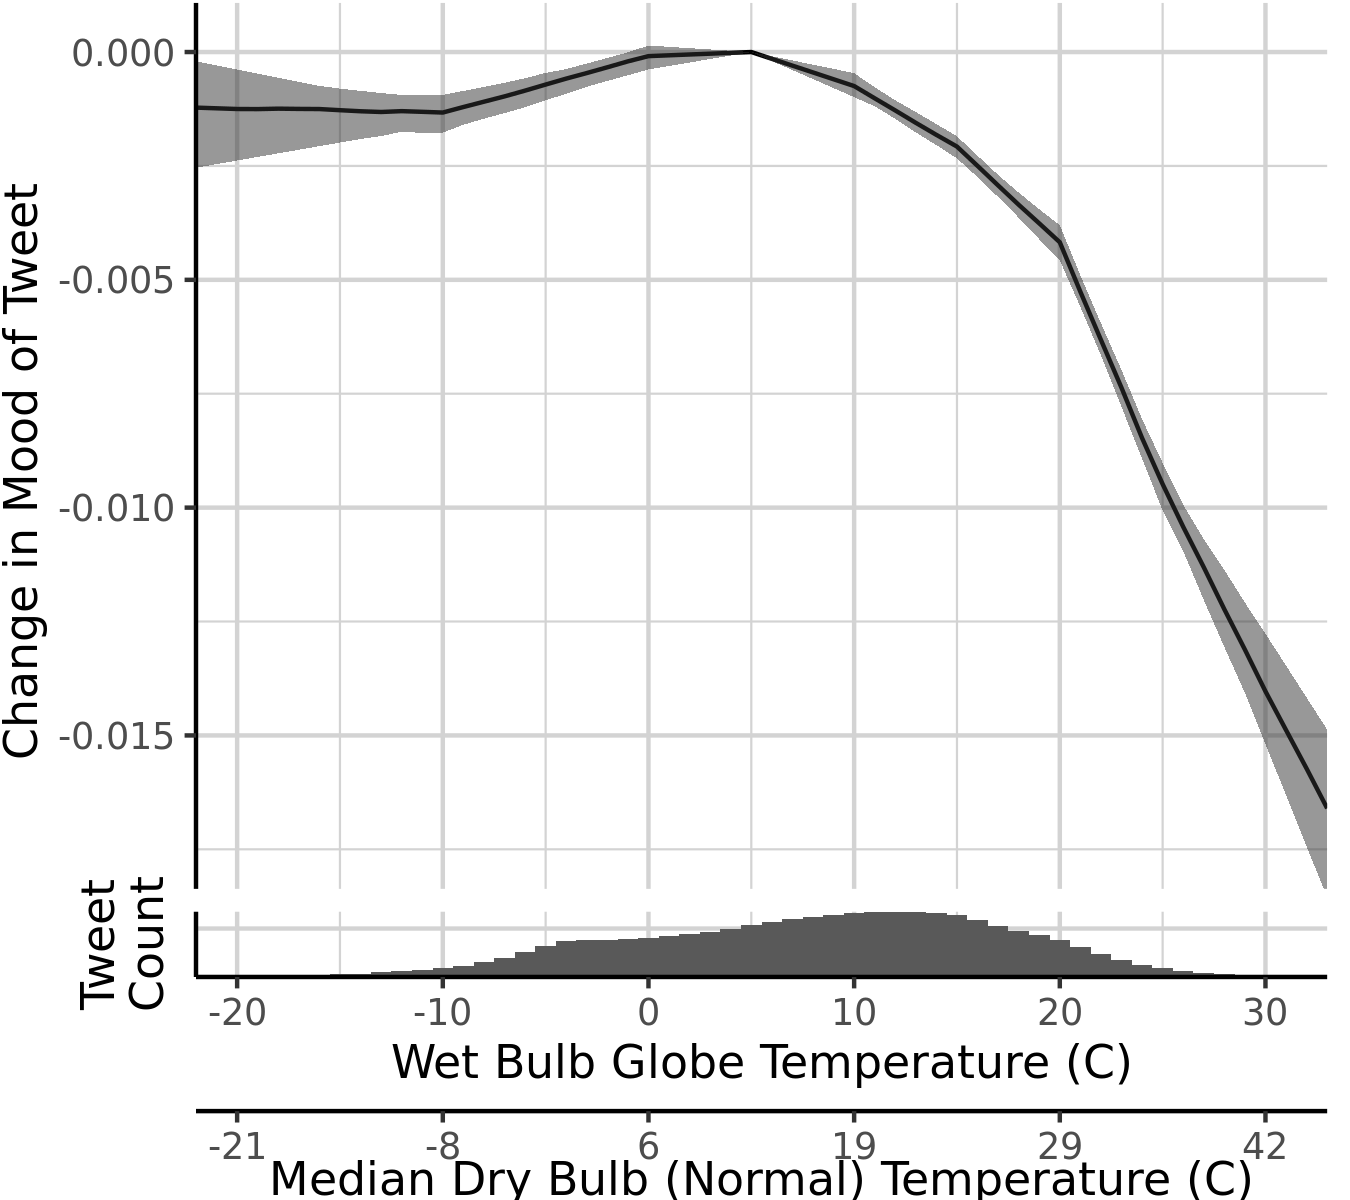
\includegraphics[width=0.5\linewidth]{../res/wbgt.png}
  \caption{Relationship between Wet Bulb Globe Temperature (WBGT) and sentiment in tweets.  As temperatures increase, sentiment declines.}
  \label{fig:wbgt}
\end{figure}

We then explored how the racial and income characteristics of neighborhoods moderate the relationship between WBGT and sentiment (See Fig \ref{fig:sub1}).  We found that neighborhood income strongly moderates the relationship between temperature and sentiment.  As temperatures increase to moderate heat of 20 WBGT (29C/84F), sentiment decreases for most neighborhoods, but increases in neighborhoods in the 95th income percentile.  These rich do not see decreases in sentiment until temperatures are above 20 WBGT (29C/84F), at which point sentiment decreases evenly across income ranges, still leaving a large gap in expressed sentiment from low to high-income neighborhoods.

We examined patterns of temperature and sentiment for neighborhoods that had a majority population of four broad racial categories - non-hispanic black, non-hispanic white, hispanic of any race, and other, which includes native american, multi-racial, and asian-american and pacific islander.  While people in neighborhoods of all racial compositions were affected by heat, people in majority black neighborhoods were much more affected than others  (See Fig \ref{fig:sub2}).  Relative to an optimum temperature of 5 WBGT (12C/54F), as temperatures increase to 30 WBGT (42C/108F), the sentiment of tweets in majority black neighborhoods decreases four-times as much as people in other neighborhoods.  Additionally, at levels of moderate heat from 10 WBGT (19C/66F) to 25 WBGT (36C/97F), people in majority hispanic neighborhoods have slightly lower sentiment than people in majority white or other neighborhoods, although this gap closes with high temperatures.

\begin{figure}[H]
\centering
\begin{subfigure}{.5\textwidth}
  \centering
  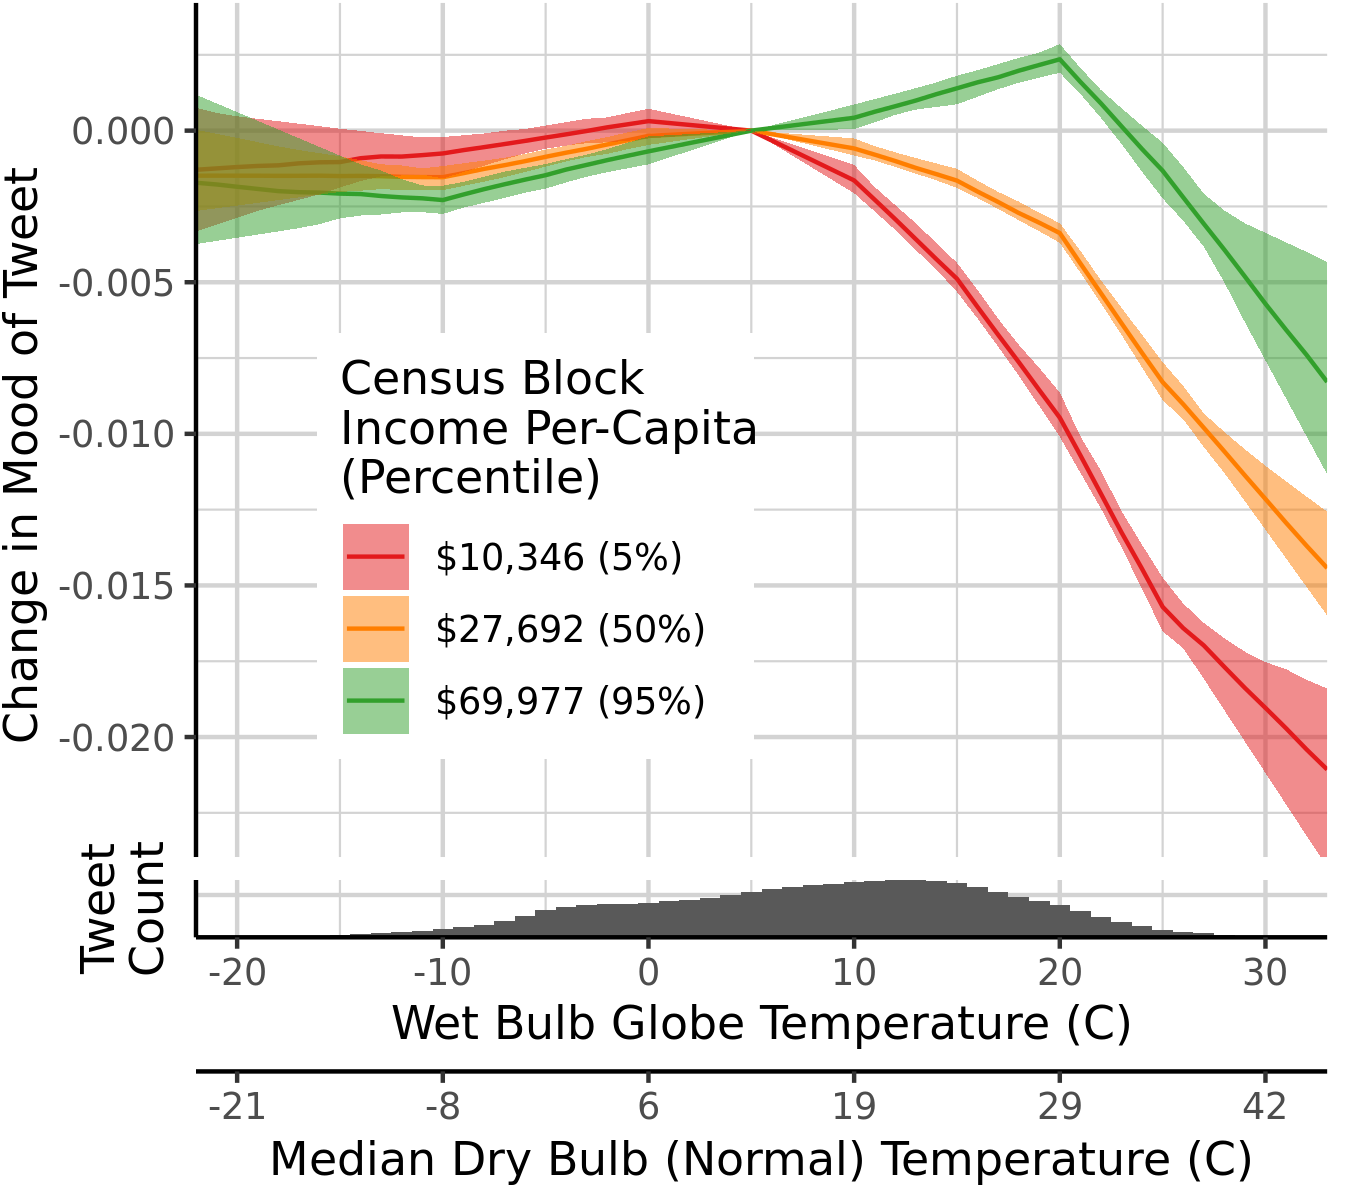
\includegraphics[width=\linewidth]{../res/wbgt-income.png}
  \caption{}
  \label{fig:sub1}
\end{subfigure}%
\begin{subfigure}{.5\textwidth}
  \centering
  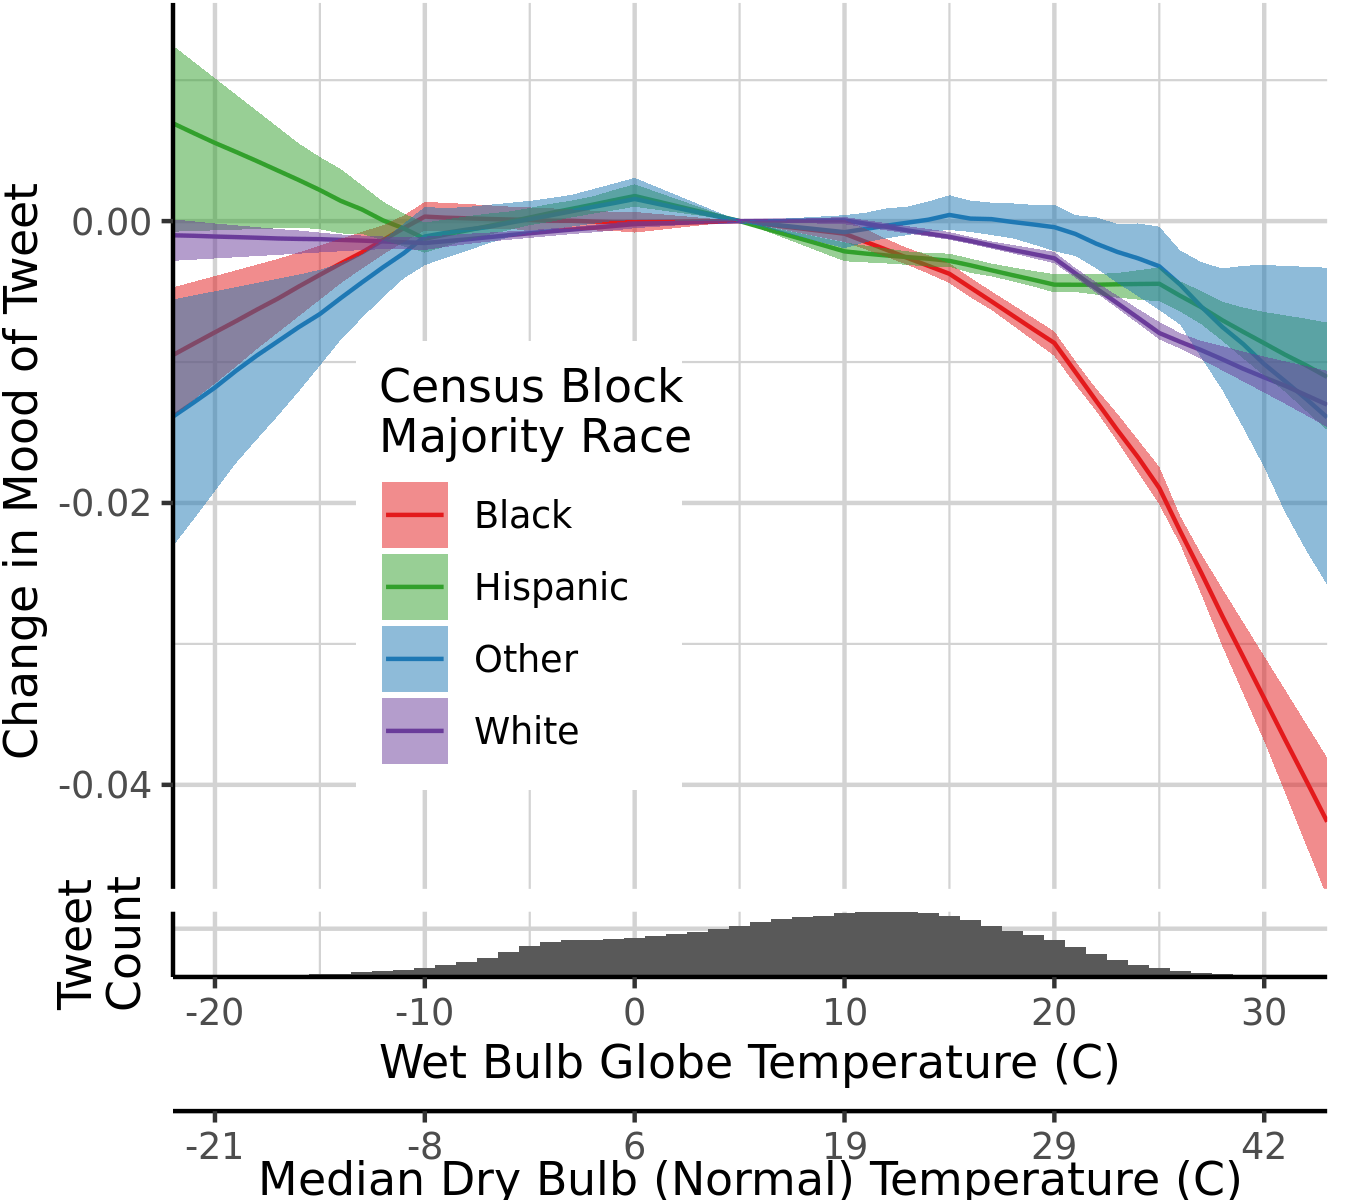
\includegraphics[width=\linewidth]{../res/wbgt-race_q.png}
  \caption{}
  \label{fig:sub2}
\end{subfigure}
\caption{Effect of changes in wet-bulb globe temperature on expressed sentiment relationship as moderated by neighborhood income (a) and race (b).}
\label{fig:test}
\end{figure}


\subsection{Comparison With Other Events}

Expressed sentiment is a widely used metric to assess mental health and well-being on social media.  While, a variety of related metrics can be used to quantify sentiment, we chose to use the VADER metric that was specifically designed for microblogs like twitter \cite{hutto2014vader}.  To give context to this metric, we compare the impacts of heat waves, defined as a change from 5 WBGT (12C/54F) to 25 WBGT (36C/97F), to the change in average sentiment from Saturday to Monday as well as the impacts on of the two most expensive hurricanes in the last decade in the United States (See Fig. \ref{fig:compare}.  Saturday and Monday are the highest and lowest days for both twitter sentiment and suicides, and over the course of our study period, Mondays had 23\% more suicides than Saturdays.  For the hurricanes, we compared the mean sentiment of counties affected by Hurricanes Harvey and Sandy on the day of landfall to the mean sentiment a week before.  These hurricanes are associated with mental health effects including Post-Traumatic Stress Disorder (PTSD) \cite{Schwartz2017Aug, Schwartz2018May}, and similar disasters have been associated with subsequent increases in suicides \cite{Krug1998Feb}.

\begin{figure}[H]
  \centering
  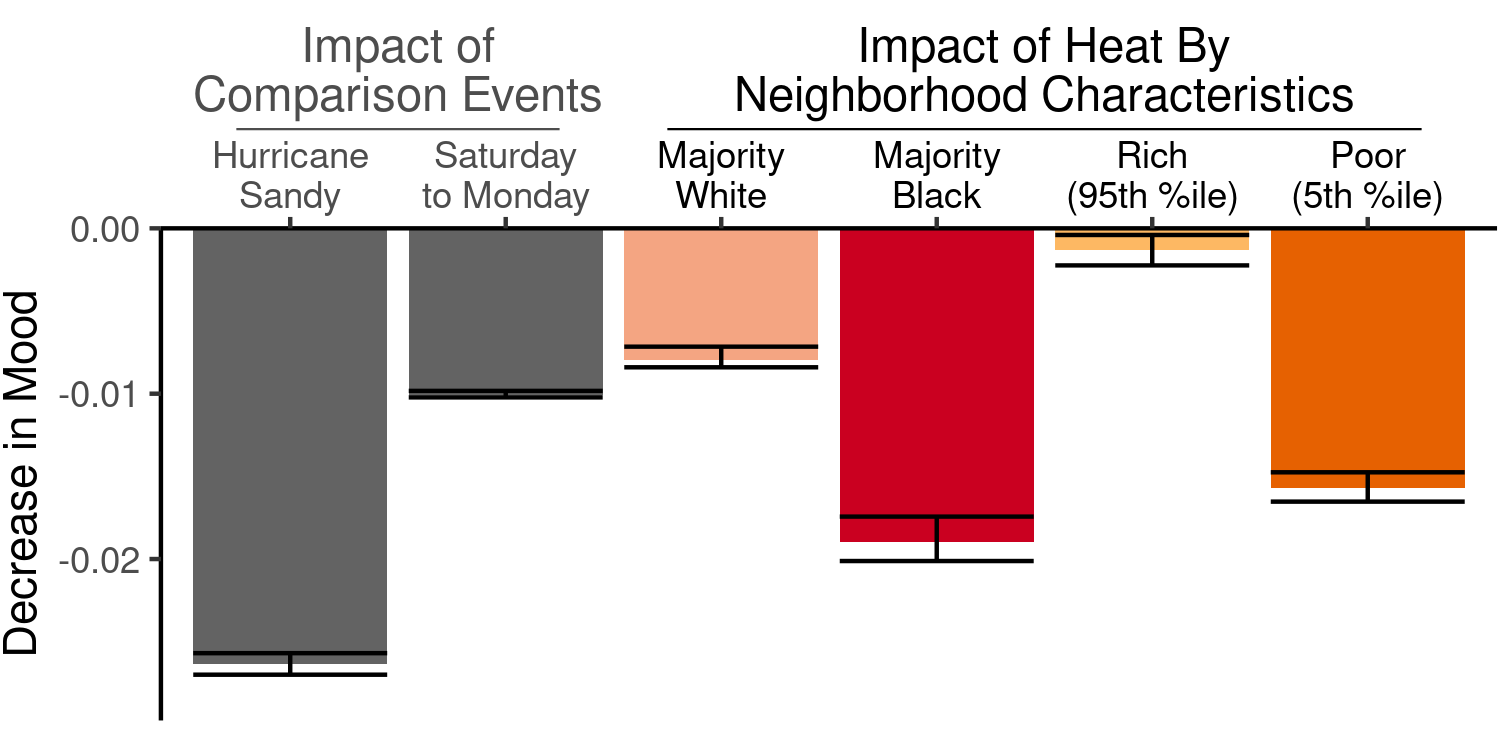
\includegraphics[width=\linewidth]{../res/comparison_plot.png}
  \caption{Decline in sentiment during a heat wave across several different neighborhoods, compared with other impacts on sentiment, such as major hurricanes, as well as the weekly variation in sentiment from the peak on Saturday to the low on Monday.}
  \label{fig:compare}
\end{figure}

We found that the impacts of heatwaves on sentiment in rich and majority white neighborhoods were less than the average weekly change in sentiment from Saturday to Monday, but the effects of heat waves on majority black or poor neighborhoods were much greater than the average weekly change in sentiment.  Additionally, the impacts of heat waves more vulnerable neighborhoods were near to the impacts of Hurricane Sandy.

{\color{red} What other disasters/comparison events should we look at?}

\subsection{Effects by Combined Statistical Area}

To further explore our findings, we examined inequalities in the impacts of higher temperatures on sentiment by Combined Statistical Areas (CSAs) and Metropolitan Statistical Areas (MSAs) with over 1 million people (hereafter: cities).  We examined the change in size of the gap in sentiment scores between both poor and rich neighborhoods, as well as black and non-black neighborhoods, as temperatures change from optimum temperatures of 5 WBGT (12C/54F) to 30 WBGT (42C/108F).

We found increasing inequalities in sentiment across income groups for 68.8\% of cities, with 35.6\% of these having a statistically significant effect (15 cities).  Cities with a significantly unequal effect were found in the south, midwest, northeast, northwest, and southwest, although they were most common in the mid-atlantic region.  Additionally, many cities in the southwest had an inverted effect, where higher temperatures actually narrowed the gap in sentiment between rich and poor neighborhoods, including Denver and Oklahoma City, which had a statistically significant inverted effect.

Because we found a much stronger effect for the effects of temperature on sentiment in majority black neighborhoods, we also examined increases in sentiment gaps between black and non-black neighborhoods in cities with a black population greater than 5\% of the total population.  We found increasing inequalities in sentiment for more black neighrborhoods in 64.7\% of cities, with a significant effect in 21.2\% of those (7 cities).  Additionally, three sunbelt cities had a significant inverted effect.  The patterns of inequalities in the impacts of heat on sentiment by race were similar to inequalities by income: cities with large and significant inequalities were found the mid-atlantic and midwest, as well as central florida.

\begin{figure}[H]
\centering
\begin{subfigure}{0.75\textwidth}
  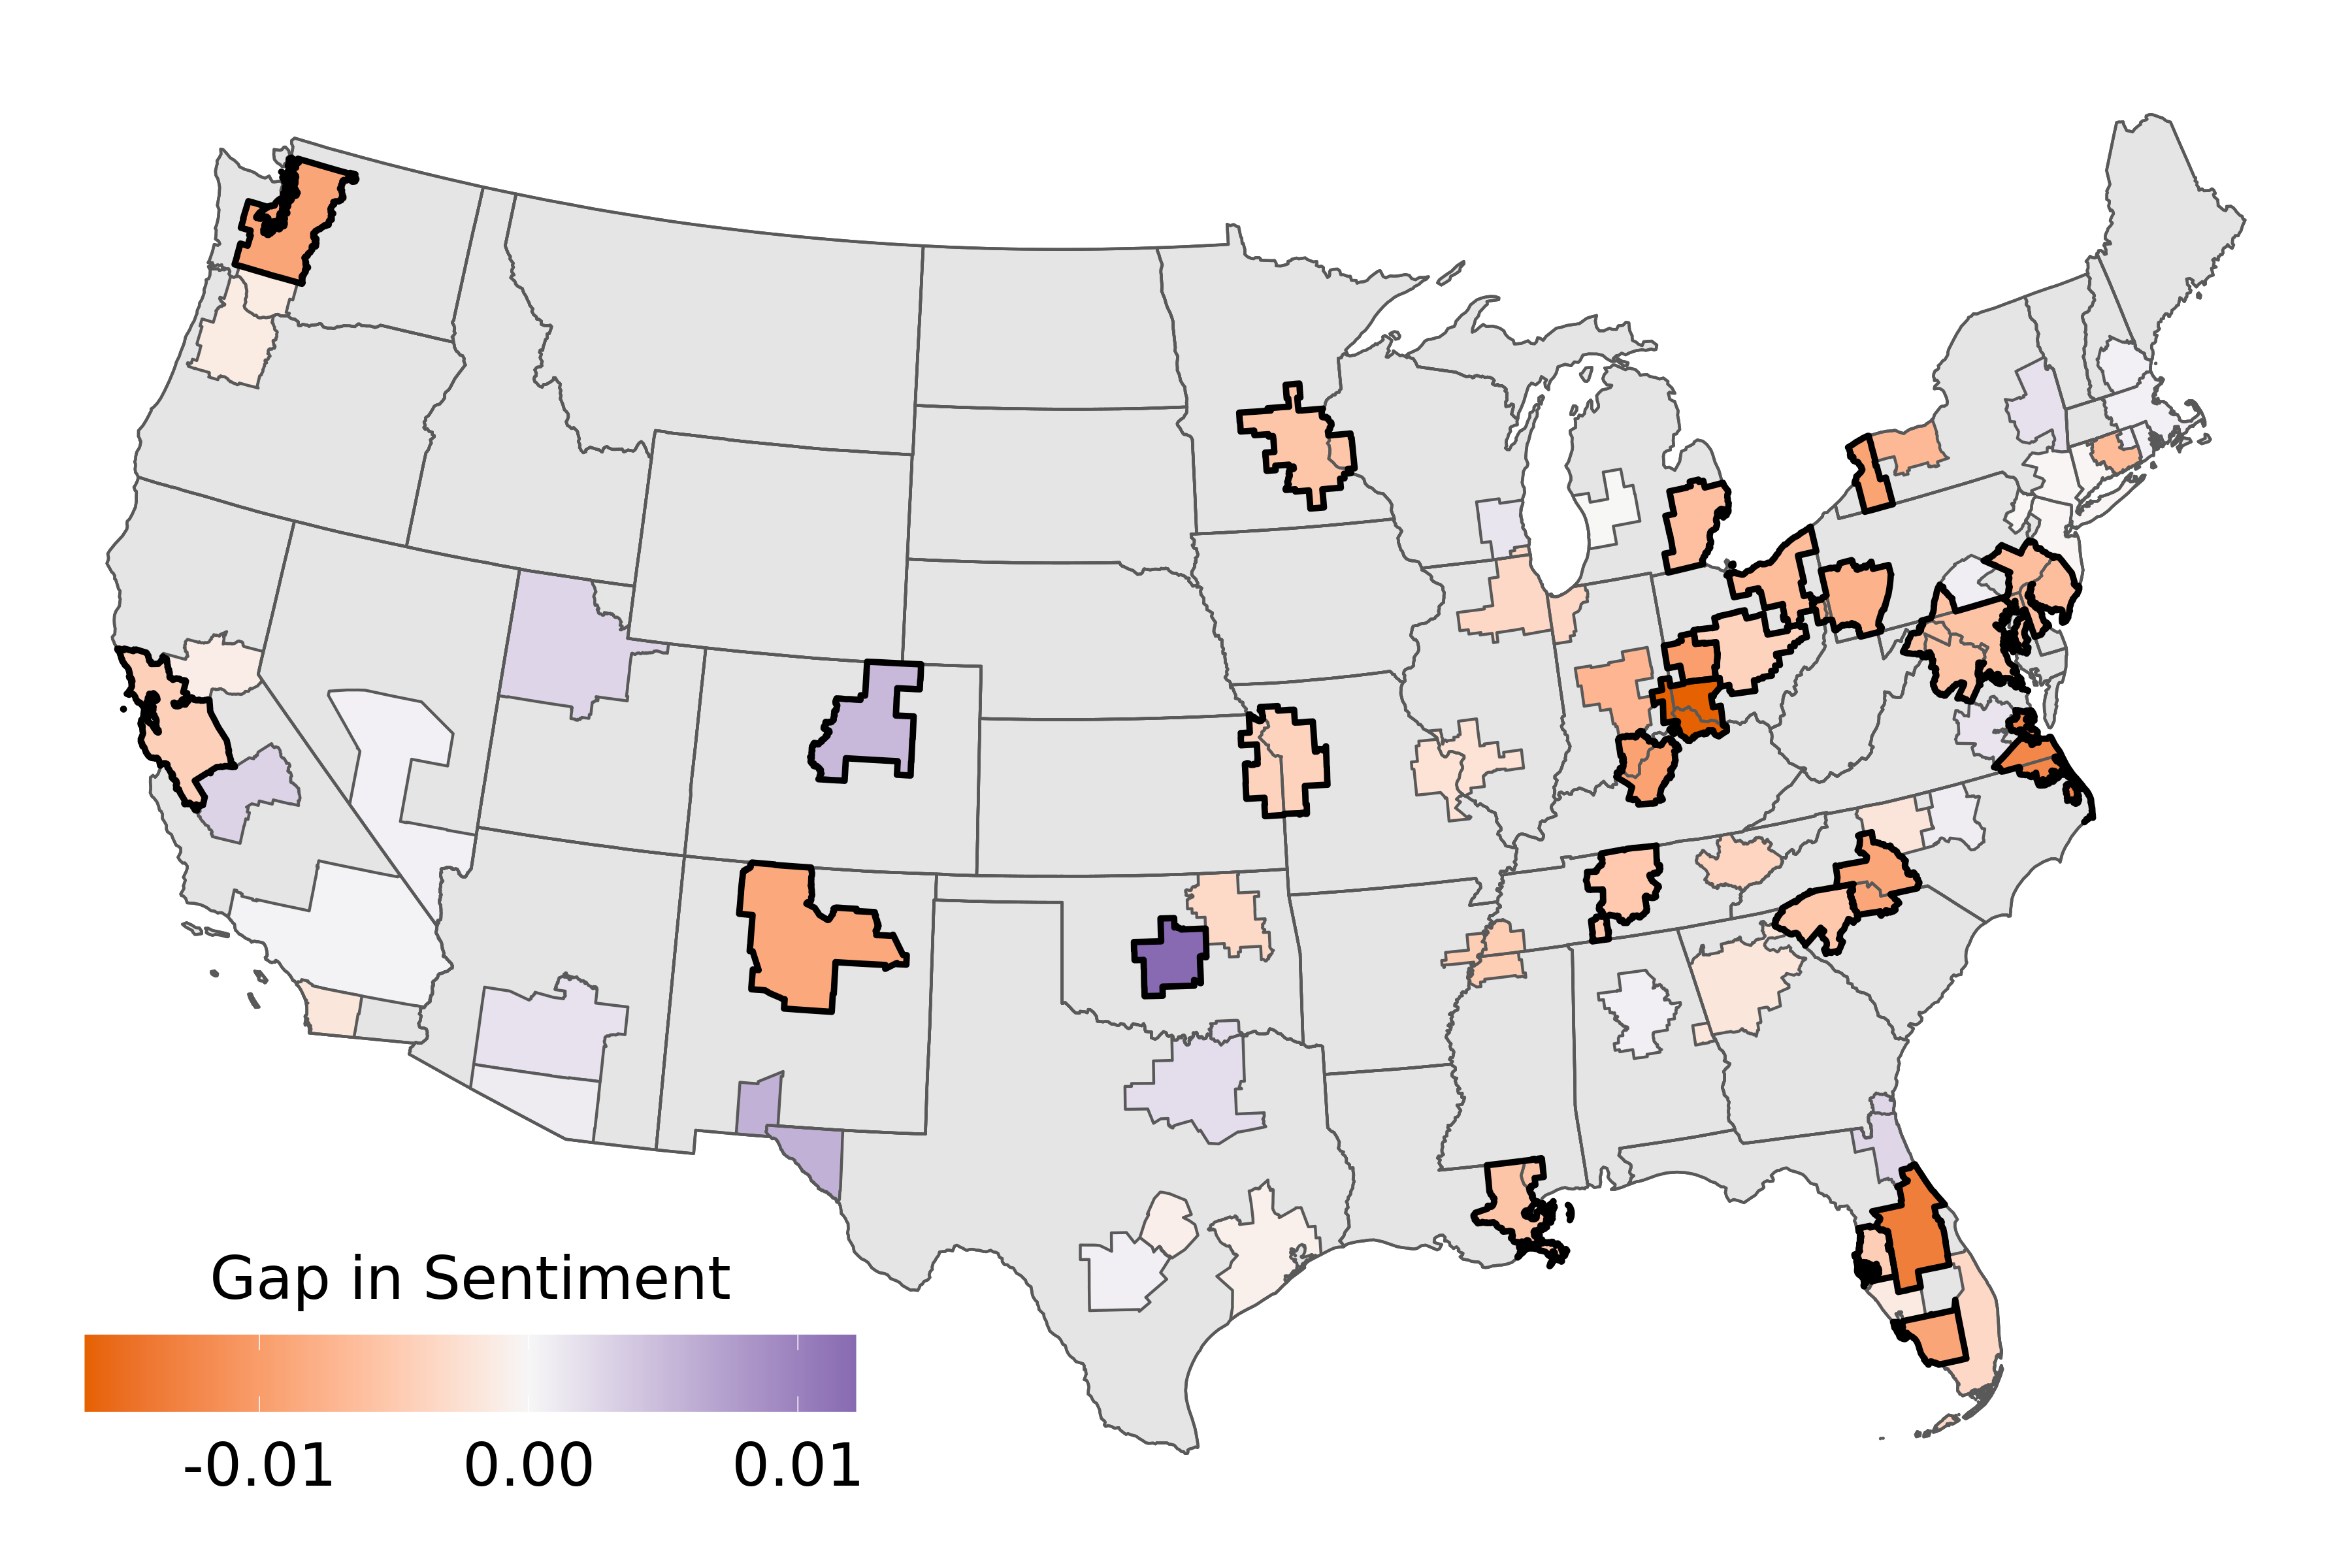
\includegraphics[width=\linewidth]{../res/map_wbgt_income.png}
  \caption{}
  \label{fig:map1}
\end{subfigure}
\begin{subfigure}{0.75\textwidth}
  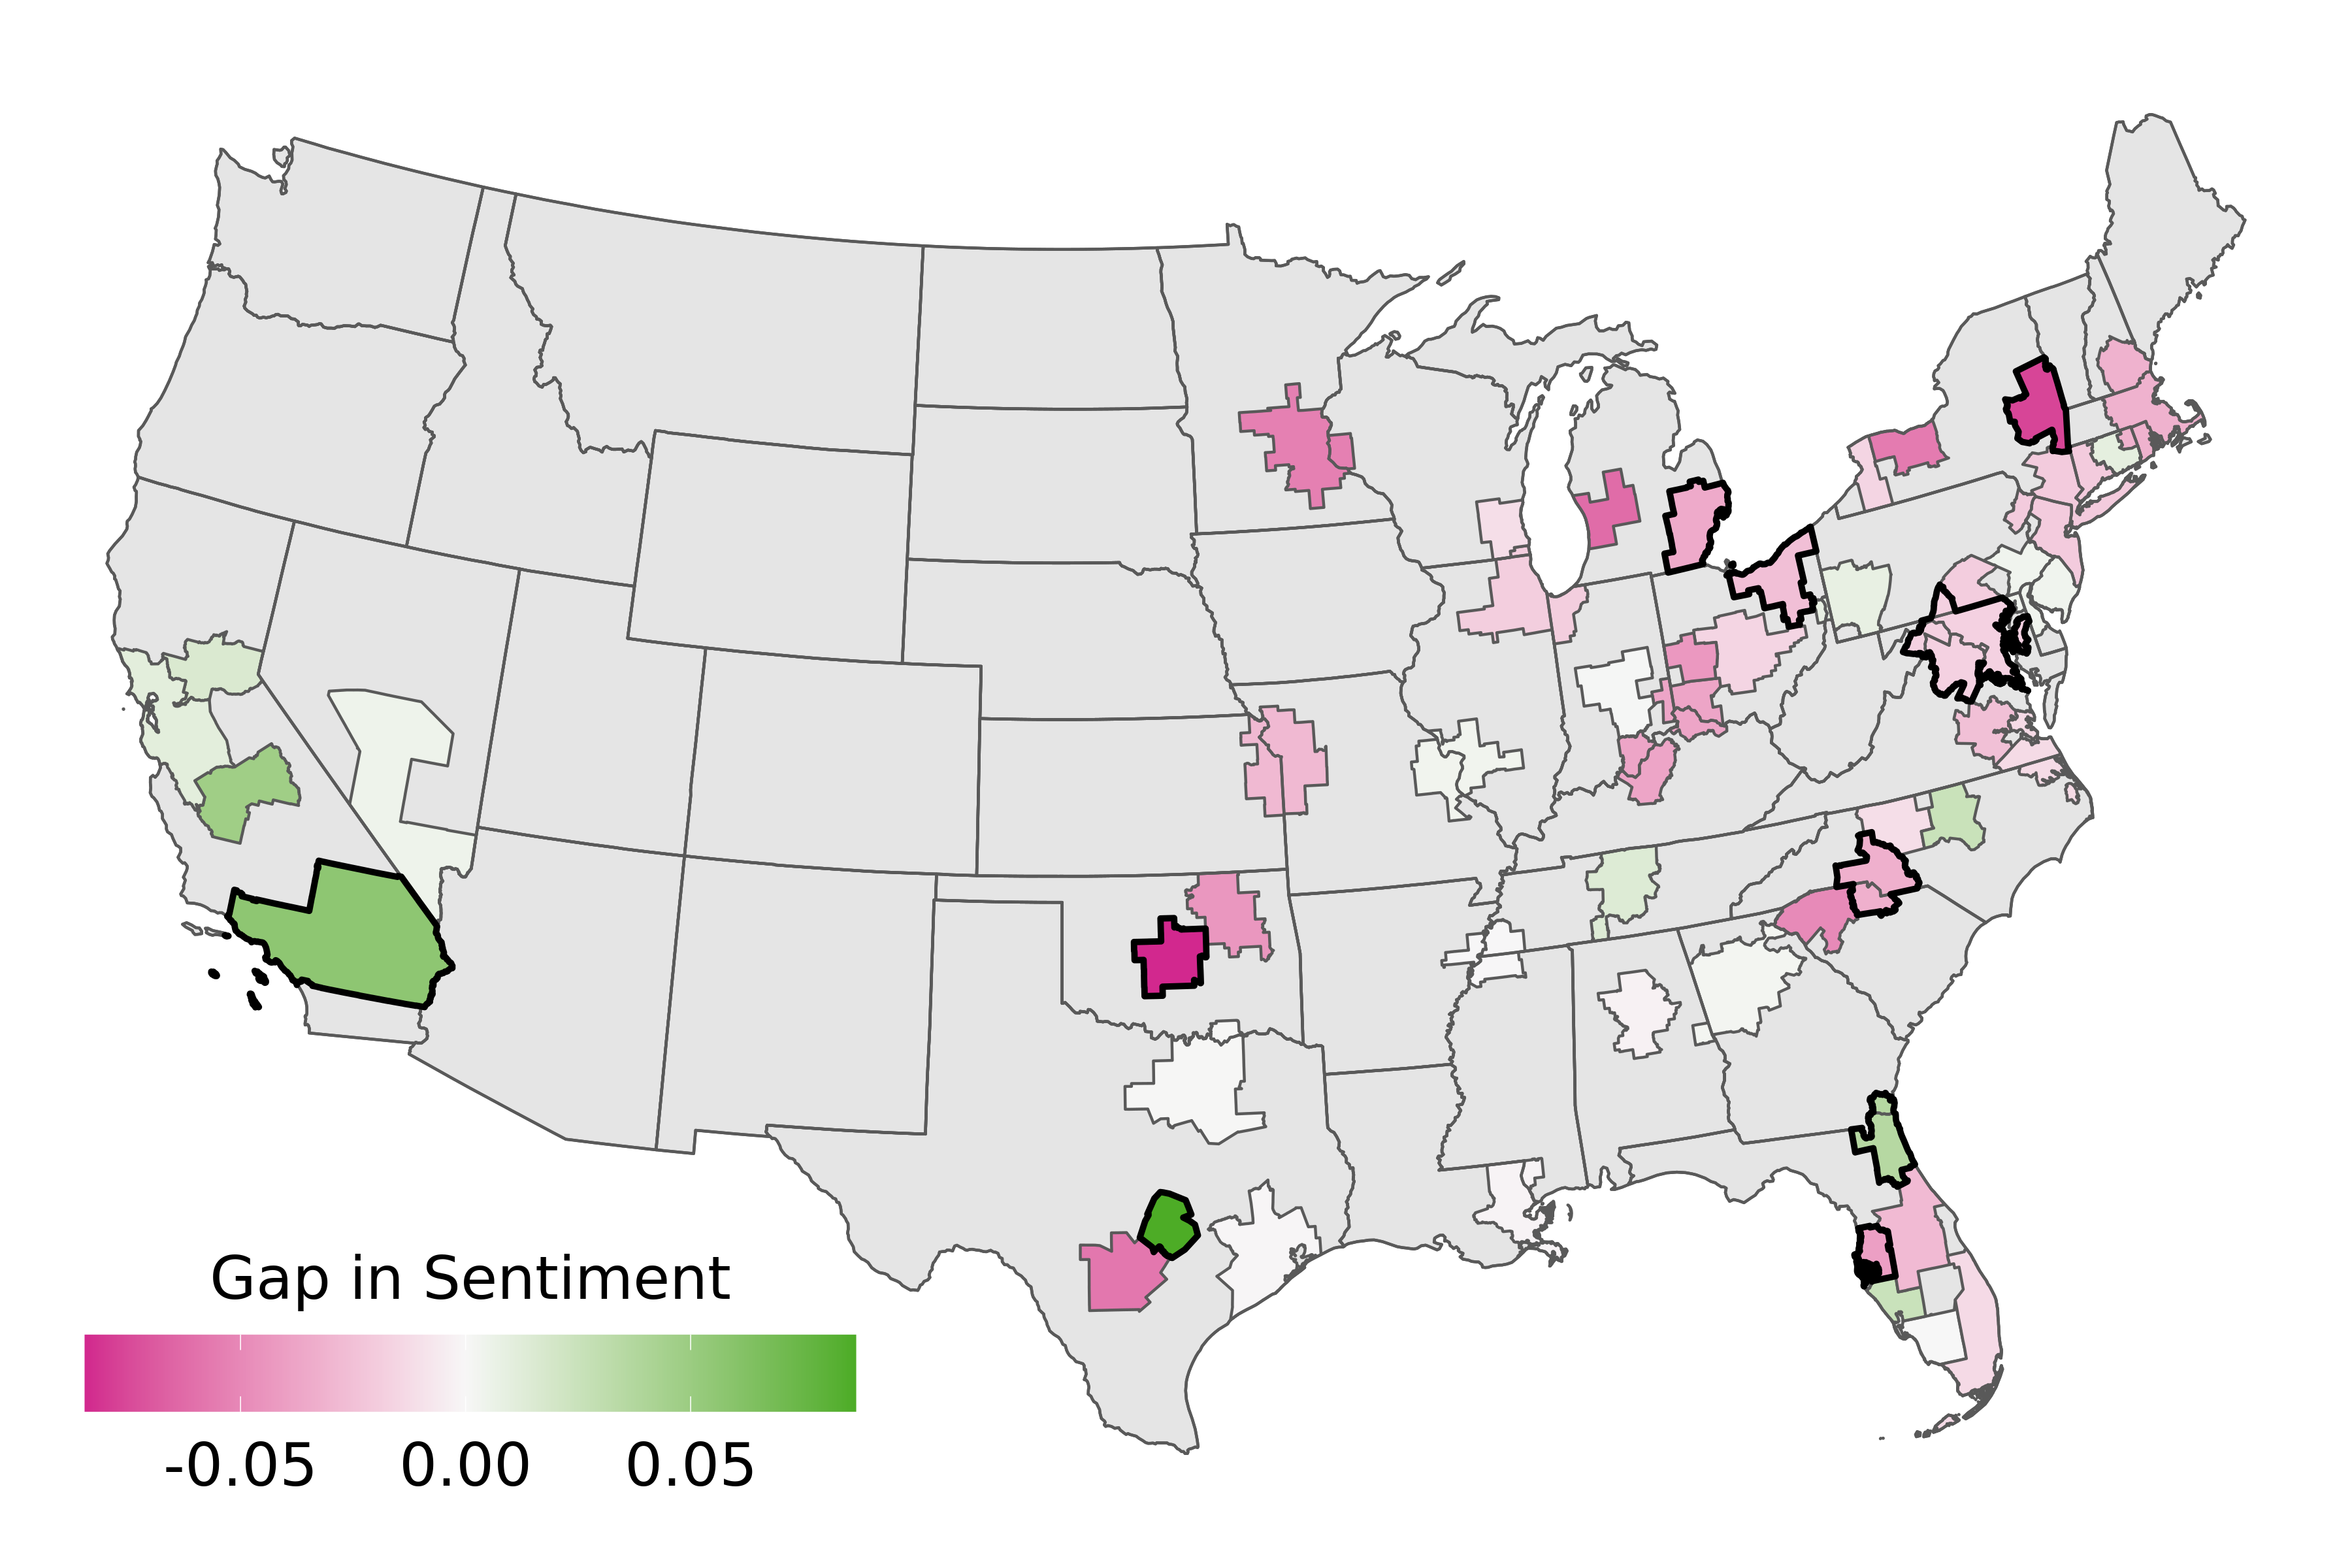
\includegraphics[width=\linewidth]{../res/map_wbgt_black.png}
  \caption{}
  \label{fig:map2}
\end{subfigure}
\caption{Inequalities in impacts of temperature on sentiment by CSAs and MSAs with over 1 million people.  The value shown is the predicted change in the size of the gap in vader score as temperatures increase from 5 WBGT to 30 WBGT between the 5th and 95 percentile for income (a) and the 95th and 5th percentile for percent black (b).  CSAs with a statistically significant effect ($p < 0.05$) are outlined in black.  For racial inequalities (b), only MSAs and CSAs where black people make up >5\% of the population are included.}
\label{fig:test}
\end{figure}

\subsection{Effects by Time of Day}

In addition to providing data with high spatial resolution, twitter data also comes with very high temporal resolution as each tweet is time-stamped.  Thus, we were able to examine the impact of heat on sentiment for each hour of the day (See Fig. \ref{fig:ts-wbgt}).  We found that heat decreased expressed sentiment at nearly all hours of the day, and that heat had the largest effect on sentiment early in the morning, between 4am and 6am.  Heat had the weakest effects on sentiment at midday, and at 3am.

\begin{figure}[H]
  \centering
  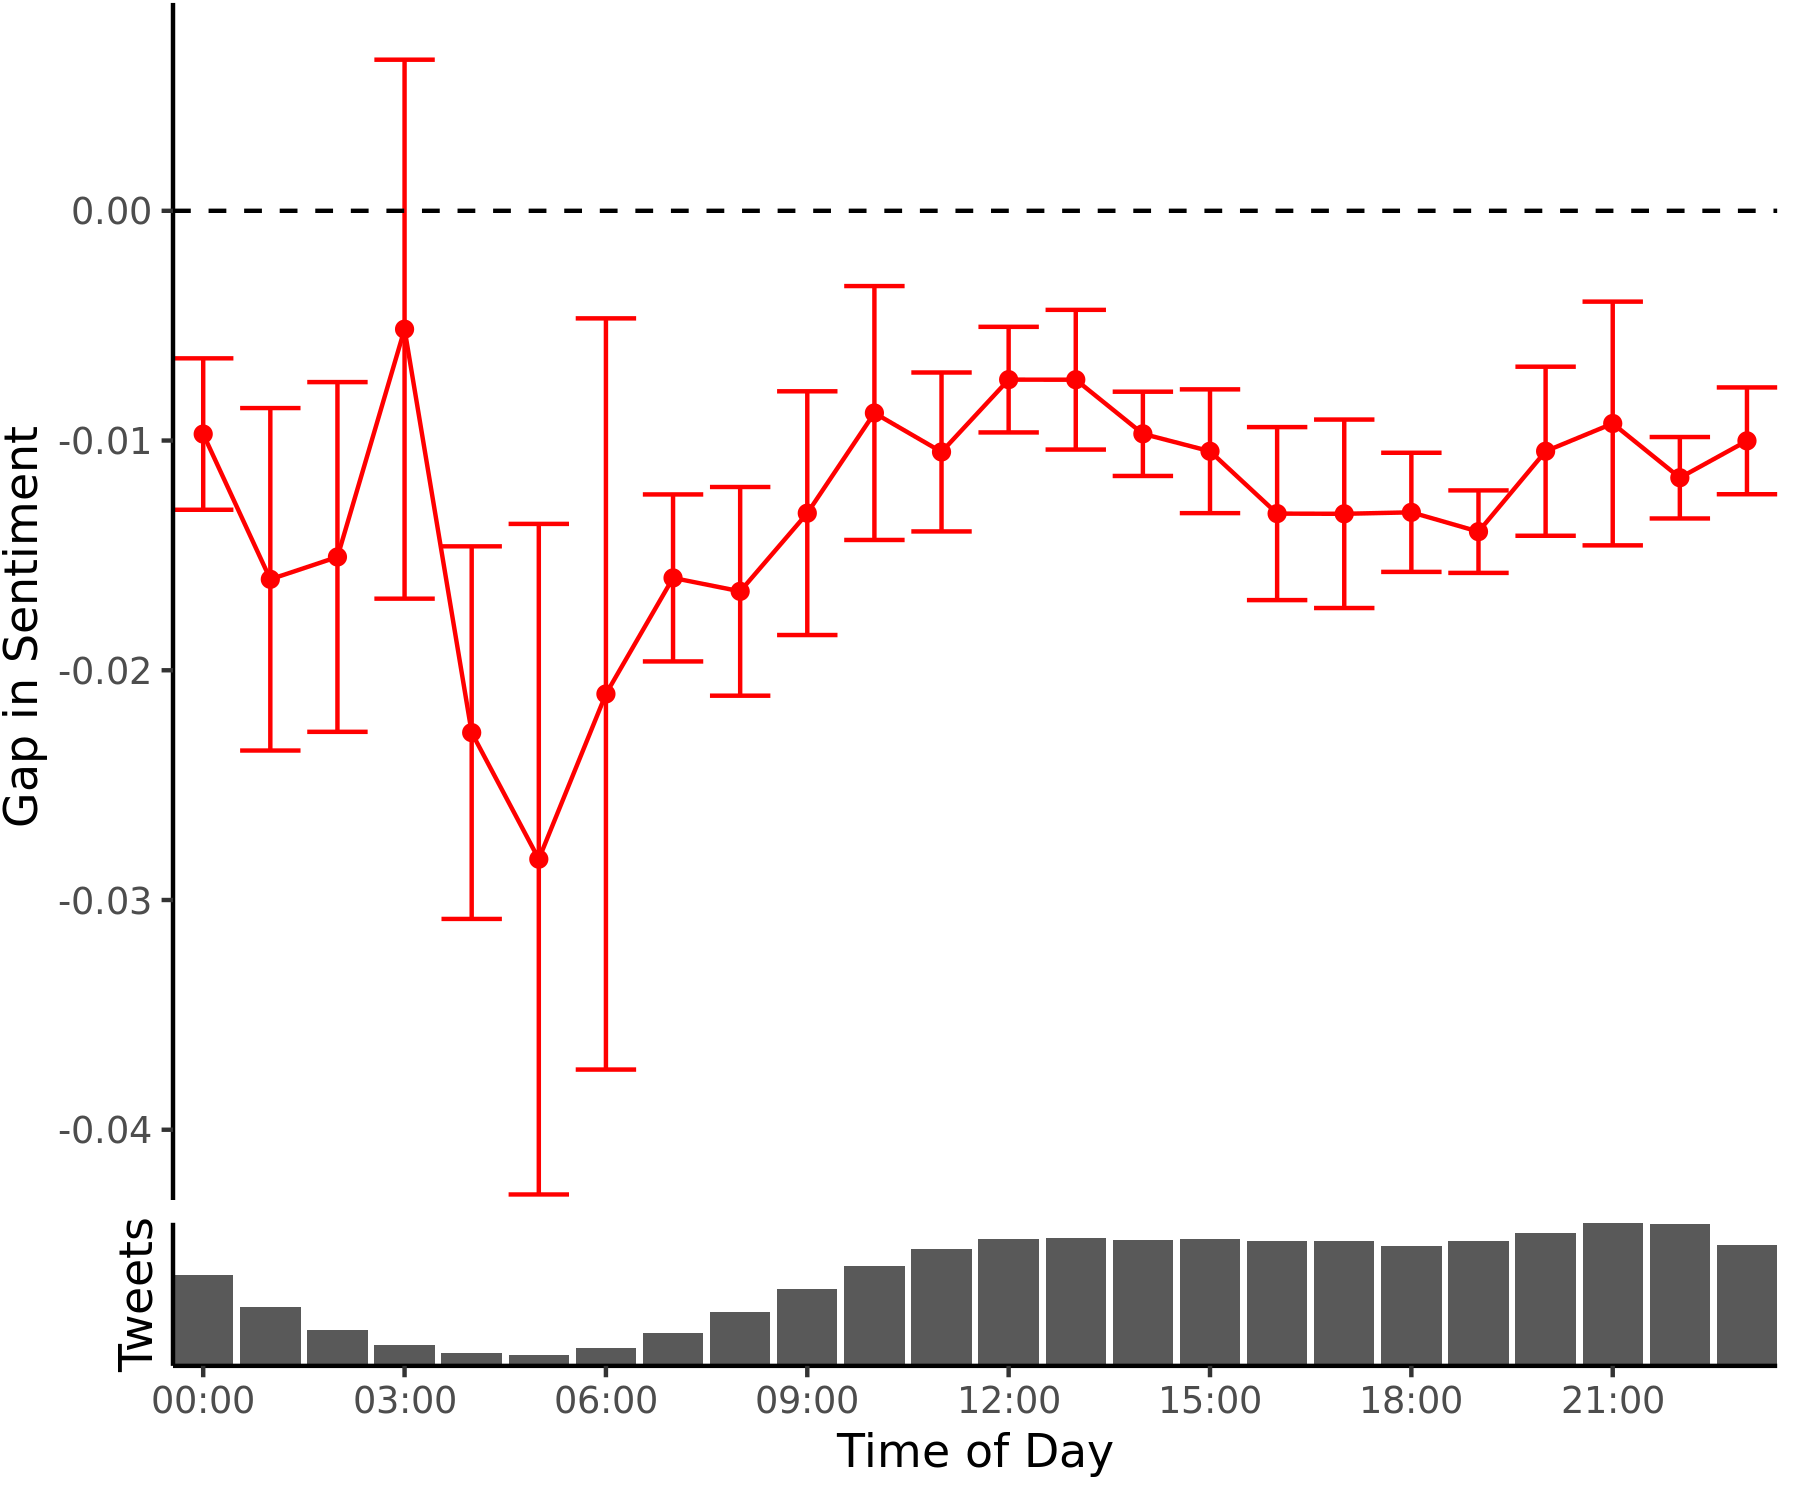
\includegraphics[width=0.75\linewidth]{../res/ts.png}
  \caption{Effects of rising temperatures on sentiment by hour of the day, with a 95\% confidence interval.  The value shown is the predicted change in vader score for a 25-degree increase in temperatures.}
  \label{fig:ts-wbgt}
\end{figure}

\section{Discussion}
We found that twitter data offers significant advantages for observing environmental effects on human well-being due to its very fine spatio-temporal resolution.  We were able to pair each tweet with the local temperature at the time of the tweet, and found a clear association between heat and worsened sentiment.   Moreover, we were able to show clear heterogeneities in vulnerability by neighborhood characteristics, overturning previous findings that found no heterogeneities at the county level \cite{Burke2018Aug, Mullins2019Dec}.

However, one limitation of data from twitter is that a tweet is not a precise measurement of a mental health outcome, but rather only a rough indicator a user's mental state based on the vocabulary in the tweet.  Moreover, while sentiment analysis algorithms have gotten increasingly sophisticated at estimating the mood in a body of text, accounting for negations (``\textit{not} good"), punctuation (``Good!!!"), emoticons and emojis (":-) or d grin




% This could honestly be its own appendix section
  The change from optimum temperature of 5WBGT (12C/54F) to a heatwave of 25WBGT (36C/97F) is associated with an overall decrease in the vader sentiment score of 0.01.  This is similar to the degree of change in sentiment over the course of a week from a Monday nadir (0.1268) to a Saturday peak (0.1372).  Additionally, over the study period from 2009-2019, suicides followed a very similar weekly pattern, peaking on Mondays and declining over the course of the week until Saturday.  From Saturday to Monday, suicides increase 23\%.  Thus, while research on linkages between sentiment and other mental health outcomes like suicides and hospitalizations is still nascent, there are clear similarities in patters of sentiment at some time scales.  Moreover, both suicides and sentiment are affected by higher temperatures.  Thus, while twitter sentiments are the only mental health indicator available at fine enough spatial and temporal scales to examine neighborhood and hourly effects, these changes in sentiment are representative of real human suffering, and are also very likely indicative of medical outcomes like suicides and hospitalizations.

Recent research has suggested that the impacts of heat on sleep quality may play a large role in the observed mental health effects of heat, 
\section{Data}
A proposed list of tables and figures:
Figures for location of USA Tweets (to show aggregation and coverage).
Figures of income blocks and temperature extremes.
Table 1. Variable descriptions for what's included in our models.
Table 2. Descriptive statistics for datasets/variables we include.
Table 3. Model results with variables included in the models coefficients, SEs, p-values, sample size.
Appendix table. Sentiment scores across all types we considered.

Weird effect of southwest - WBGT means this is more likely to be cultural than due to different heat effects.


\section{Methods}
\subsection{Tweets}
We used data from 243 million geolocated tweets from the lower 48 states from the years 2009 to 2019.  

Text data used for this project come from Twitter via the University of Vermont’s (UVM) agreement with Twitter to access its streaming API - colloquially referred to as the Decahose. The "decahose" provides public access to a random 10\% of all public messages on Twitter. The UVM special agreement with Twitter allows for access to this data for research and analysis purposes and we have complied with all the terms of service for Twitter and UVM. 
The Twitter data consists of publicly posted messages, or Tweets, that are short status messages users post to the platform. We used all geolocated Tweets from the Decahose for the period 2009-2019. We only considered users’ original content, thus did not include retweets in our analysis.

We excluded all tweets that contained weather-related terms.

\subsection{Weather}
We used data on local weather conditions from the North American Land Data Assimilation System (NLDAS), a gridded product developed by several collaborative institutions, including NOAA, NASA, Princeton University, and the University of Washington.  This dataset is available at an hourly temporal resolution, and at 1/8th decimal degree spatial resolution, and integrates a large quantity of observation-based and modeled data  \cite{xia_continental-scale_2012}.  For the exact hour and location of each tweet, we extracted temperature, specific humidity, air pressure, total precipitation, shortwave radiation, and wind speed.  

Because metrics of apparent temperature that take into account humidity and other factors can better account for the impacts of heat stress on human health and wellbeing, we calculate the Wet Bulb Globe Temperature (WBGT) at the time and location of each tweet.  WBGT is the temperature that a wet globe thermometer would read in direct sunlight, and gives a reading lower than a dry bulb temperature would show due to evaporative cooling, and can be estimated given normal temperature, relative humidity, solar radiation, and wind speed.  Because evaporative cooling is how humans cool themselves through perspiration, this temperature better indicates the heat stress that people are experiencing.  Metrics like WBGT that account for the effects of humidity and other factors on heat stress have been associated with diminished economic output \cite{rao2020projections}, increased crime \cite{hu2017impact}, increased mortality \cite{chien2016spatiotemporal, armstrong2019role}, and worsened mental health outcomes \cite{vida2012relationship, ding2016importance}.

Using temperature, specific humidity, and pressure, we derived relative humidity using methods described by  \cite{bolton_computation_1980}.  We then calculated the WBGT using the formula described by \cite{heo2019comparison}.

\subsection{Socio-Econoimc Data}
We used data from the American Communit   Survey administered by the US Census to income levels and the racial composition of neighborhoods where tweets were located.  Data was at the level of the census block group, the smallest unit for which the census releases public data.

ACS data is released to cover five-year periods.  We therefore matched each tweet with census block group data from the year at the middle year of each survey's five-year range.  For example, tweets from 2014 were matched to data from the 2012-2016 ACS.  Because the most recent available data was from 2014-2018, all tweets from year years greater than 2016 were matched to this dataset.  Data was downloaded from the IPUMS NHGIS service provided by the University of Minnesota.

Mean annual income per capita is provided by the ACS, and we standardized this variable so that the values for each year were in 2019 dollars.  For racial categories, we combined the various categories provided by the ACS into four racial groups: non-Hispanic white, non-Hispanic black, Hispanic of any race, and an "other" category for non-Hispanic people who were neither black nor white, such as Asian, Native American, or mixed-race people.


\subsection{Sentiment}

WE EXCLUDED WEATHER TERMS

We assessed the sentiment expressed in text using several of the most commonly used measures of sentiment. Each of the measures uses validated dictionaries of words that have been assigned positive and negative scores and compares these words with words in the text corpora of interest. For measures of sentiment, we used the Hedonometer \href{https://hedonometer.org/timeseries/en_all/}{(link)}, Afinn \href{http://corpustext.com/reference/sentiment_afinn.html}{(link)}, Textblob \href{https://textblob.readthedocs.io/en/dev/}{(link)}, Vader , SentiwordNet and LIWC tools. These tools assign positive and negative scores to words, then average the scores for each text string. Our text data was multilingual, which can present challenges with analyzing text (cite). Given our interest only in the collection of words used (in aggregate) and not the sequence or nuance of the phrases, we translated all languages into English using Google Translate API and the Microsoft Azure API cognitive services (translator text API) before conducting the sentiment analyses.

Some papers we might cite in this section (only for multilingual work): Vilares et al. 2017 , Lo et al. 2017, Dashtipour et al. 2016.

Discuss issues with text data (gtp) - that it doesn’t capture emoticons, code switching (e.g., [good job! \#fail]), etc.

Issues with sample population (non-representative)

Issues with what people say on social media being attenuated or mismatched from actual emotional state

\subsubsection{Hedonometer}
The Hedonometer \cite{dodds_temporal_2011} is a corpus-based technique to get sentiment score from multi-lingual texts. The core steps are (1) building human evaluations of the happiness of a set of individual words, and (2)using a naive algorithm for scaling up from individual words to texts. For the English corpus, Dodds and others \cite{dodds_temporal_2011} collect 10,222 unique words and used crowd-sourcing platform Amazon Mechanical Turk to get human evaluation of happiness degree for each word in an integer scale from 1 to 9, representing a sad to happy spectrum. Score 5 represents neutral words. Each word will be calculated average score and then the word and happiness score are compiled into a dataset (labMT 1.0). Some illustrative example of words are: 

\[h_{avg} (\text{laughter}) = 8.50 \]
\[h_{avg} (\text{the}) = 4.98\]
\[h_{avg} (\text{hate}) = 2.34\]

The sentiment score for single text will be the mean happiness score for all words in the text.


\subsubsection{VADER}
The VADER sentiment corpus was proposed by Gilbert and Hutto \cite{gilbert_vader_2014} and stands for 'Valence Aware Dictionary for sentiment Reasoning'. It is is a lexicon and rule-based sentiment analysis tool that is specifically attuned to sentiments expressed in social media by incorporating lexical features common to sentiment expression in microblogs

\subsection{Modeling}
We assessed how expressed sentiment is affect by three weather variables: wet bulb globe temperature, precipitation, and sunshine.  Moreover, we modeled how neighborhood income affects the relationship between these weather variables and sentiment.

Our model takes the following form:
\begin{equation}
    y = \beta_0 + f_t(t) + f_{mt}(m t) + \beta_p p + \beta_{mp} m s + \beta_s s + \beta_{ms} m s + \Phi + \epsilon
\end{equation}

Where $y$ is the sentiment of a tweet, $t$ is the wet bulb globe temperature at the hour of the tweet, $p$ is a binary variable indicating whether it rained at the hour of the tweet, $s$ is the income shortwave radiation, or sunshine, in $W/m^2$, at the hour of the tweet, and $m$ is the log-transformed average income in the census block where the tweet originated.  We estimate the 


STANDARD ERRORS


\subsection{Data Processing}
We analyzed meteorological data using the R statistics open-source program version 3.6.2  (R Core Team 2019) using R Studio version 1.2.1335 (RStudio Team, 2019) and the raster \href{https://www.rdocumentation.org/packages/raster/versions/3.3-13}{(link)}, sp \href{https://cran.r-project.org/web/packages/sp/index.html}{(link)}, sf \href{https://cran.r-project.org/web/packages/sf/index.html}{(link)}, and stars \href{https://cran.r-project.org/web/packages/stars/index.html}{(link)} processing and geospatial packages installed. We analyized sentiment data using python version x.x.x with pandas \href{https://pandas.pydata.org/}{(link)} and numpy \href{https://numpy.org/}{(link)} packages installed. We extracted meteorological data using the geolocated coordinates from the Twitter posts (latitude and longitude). We calculated mean climatological scores (z-scores)using baseline meteorological data from 1990 to present, calculated at a quarter degree resolution, and based on the long-term averages and standard deviation. We calculated z-scores for each day and the overall annual average z-score. For text data cleaning we used the python package tweet-preprocessor \href{https://pypi.org/project/tweet-preprocessor/}{(link)} to remove all text and characters not part of the main text phrase (e.g., URLs, mentions, GIFs, etc.). We converted all dates and times to UTC format.

[NEED SOME TEXT ABOUT GOOGLE EARTH ENGINE AND MICROSOFT AI FOR EARTH] We conducted all data analyses on Microsoft AI for Earth's online cloud-computing environment using a combination of existing data analysis packages and scripts we developed. We used GitHub as a repository for all scripts we used in this project (link to the Git repo). To run ABC analysis, we used Microsoft's CBA package. To run XYZ analysis, we used Microsoft's ZYX package. 

%%KEY POINTS TO DISCUSS

% Link between twitter mood and other very bad outcomes (crime, suicide)

% Baselines: this could also be interpreted as: poor are less affected by the cold\textbf{:}

% Caveats:
    % Uncertainties from census blocks (low income, young areas).  This is why we used a linaer effect instead of a binned effect.
    % We cant speak to types of mental heath that are worsening - depression, anxiety, and post-traumatic stress, etc.  Just a general overview

% More nuanced interpretation: optimal temperature for poor & minority neighborhoods are much lower.

\section{Conclusion}

\section{Acknowledgements}
This work was supported by the National Socio-Environmental Synthesis Center (SESYNC) under funding received from the National Science Foundation DBI-1639145.  Additionally, cloud resources for this project were provided for the Microsoft Azure cloud by Microsoft's AI for Earth program, grant number .

\printbibliography

\end{document}

\end{document}
